\documentclass[10pt, compress]{beamer}


\PassOptionsToPackage{export}{adjustbox}
\usepackage{
  bm, 
  tikz, 
  tikzscale, 
  float, subfloat,
  caption, subcaption,
  fancybox,
  xmpmulti,
  empheq,
  framed,
}
\usetikzlibrary{fit, positioning, bayesnet}
\usepackage[mode=buildnew]{standalone}
%\usepackage[export]{adjustbox}
\usepackage{booktabs}
\usepackage[scale=2]{ccicons}
\usefonttheme[onlymath]{serif}
\usepackage{pdfpcnotes}

%\usemintedstyle{trac}

\title{Bayesian learning of structured embeddings}
\subtitle{Thesis proposal}
\date{May 11, 2018}
\author{Sharad Vikram}
\institute{UCSD}

%\setcounter{tocdepth}{1}
\usepackage{
    algorithm,algorithmic,amsfonts,amsmath,amssymb,bm,booktabs,color,
    enumerate,graphicx,hyperref,microtype,multicol,natbib,nicefrac,url
}
\usepackage[T1]{fontenc}
\usepackage[utf8]{inputenc}

\newcommand{\todo}[1]{\noindent\textbf{\textcolor{red}{(TODO) #1\\}}}

\newcommand{\MDP}{M}
\newcommand{\States}{\mathcal{S}}
\newcommand{\Actions}{\mathcal{A}}
\newcommand{\cost}{C}
\newcommand{\initstatedist}{\rho}
\newcommand{\discount}{\gamma}
\newcommand{\numsamp}{N}
\newcommand{\horizon}{T}
\newcommand{\dynamics}{p}
\newcommand{\policyparams}{\theta}
\newcommand{\policy}{\pi}
\newcommand{\state}{\mathbf{s}}
\renewcommand{\action}{\mathbf{a}}
\newcommand{\costsample}{c}
\newcommand{\policyobj}{\eta}
\newcommand{\dynmodel}{\hat{\dynamics}}
\newcommand{\costmodel}{\hat{\cost}}
\newcommand{\isdmodel}{\rho}
\newcommand{\dynmat}{\mathbf{F}}
\newcommand{\dyncovar}{\Sigma}
\newcommand{\costmat}{\mathbf{C}}
\newcommand{\costvec}{\mathbf{c}}
\newcommand{\K}{\mathbf{K}}
\renewcommand{\k}{\mathbf{k}}
\newcommand{\polcovar}{\mathbf{S}}
\newcommand{\latent}{\mathbf{x}}
\newcommand{\traj}{\tau}
\newcommand{\polstepsize}{\epsilon_p}
\newcommand{\modelstepsize}{\epsilon_m}
\newcommand{\R}{\mathbb{R}}
\newcommand{\N}{\mathcal{N}}
\newcommand{\NIW}{\mathcal{NIW}}
\newcommand{\W}{\mathcal{W}}
\renewcommand{\L}{\mathcal{L}}
\newcommand{\E}{\mathbb{E}}
\newcommand{\I}{\mathbb{I}}
\newcommand{\KL}{\textrm{KL}}
\newcommand{\model}{\mathcal{M}}
\newcommand{\dataset}{\mathcal{D}}
\DeclareMathOperator*{\argmin}{argmin}
\DeclareMathOperator*{\argmax}{argmax}
\newcommand{\colvec}[2][.67]{%
  \scalebox{#1}{%
    \renewcommand{\arraystretch}{.67}%
    $\begin{bmatrix}#2\end{bmatrix}$%
  }
}
\newcommand{\trajectory}{\left[\state_0,\action_0,\ldots,\state_\horizon,\action_\horizon,\state_{\horizon + 1}\right]}
\newcommand{\costtrajectory}{\left[\state_0,\action_0,\costsample_0\ldots,\state_\horizon,\action_\horizon,\costsample_\horizon,\state_{\horizon + 1}\right]}
\newcommand{\latenttrajectory}{\left[\latent_0,\action_0,\ldots,\latent_\horizon,\action_\horizon,\latent_{\horizon + 1}\right]}

\usetheme{metropolis}           % Use metropolis theme

\begin{document}

\begin{frame}
  \titlepage
\end{frame}

\section{Overview}

\begin{frame}{Unsupervised learning}
  \begin{columns}[T]
    \begin{column}{0.5\textwidth}
      \begin{overlayarea}{\textwidth}{7cm}
        \begin{center}
          \Large \textbf{Structure}\\ \vspace{10pt}
        \only<1>{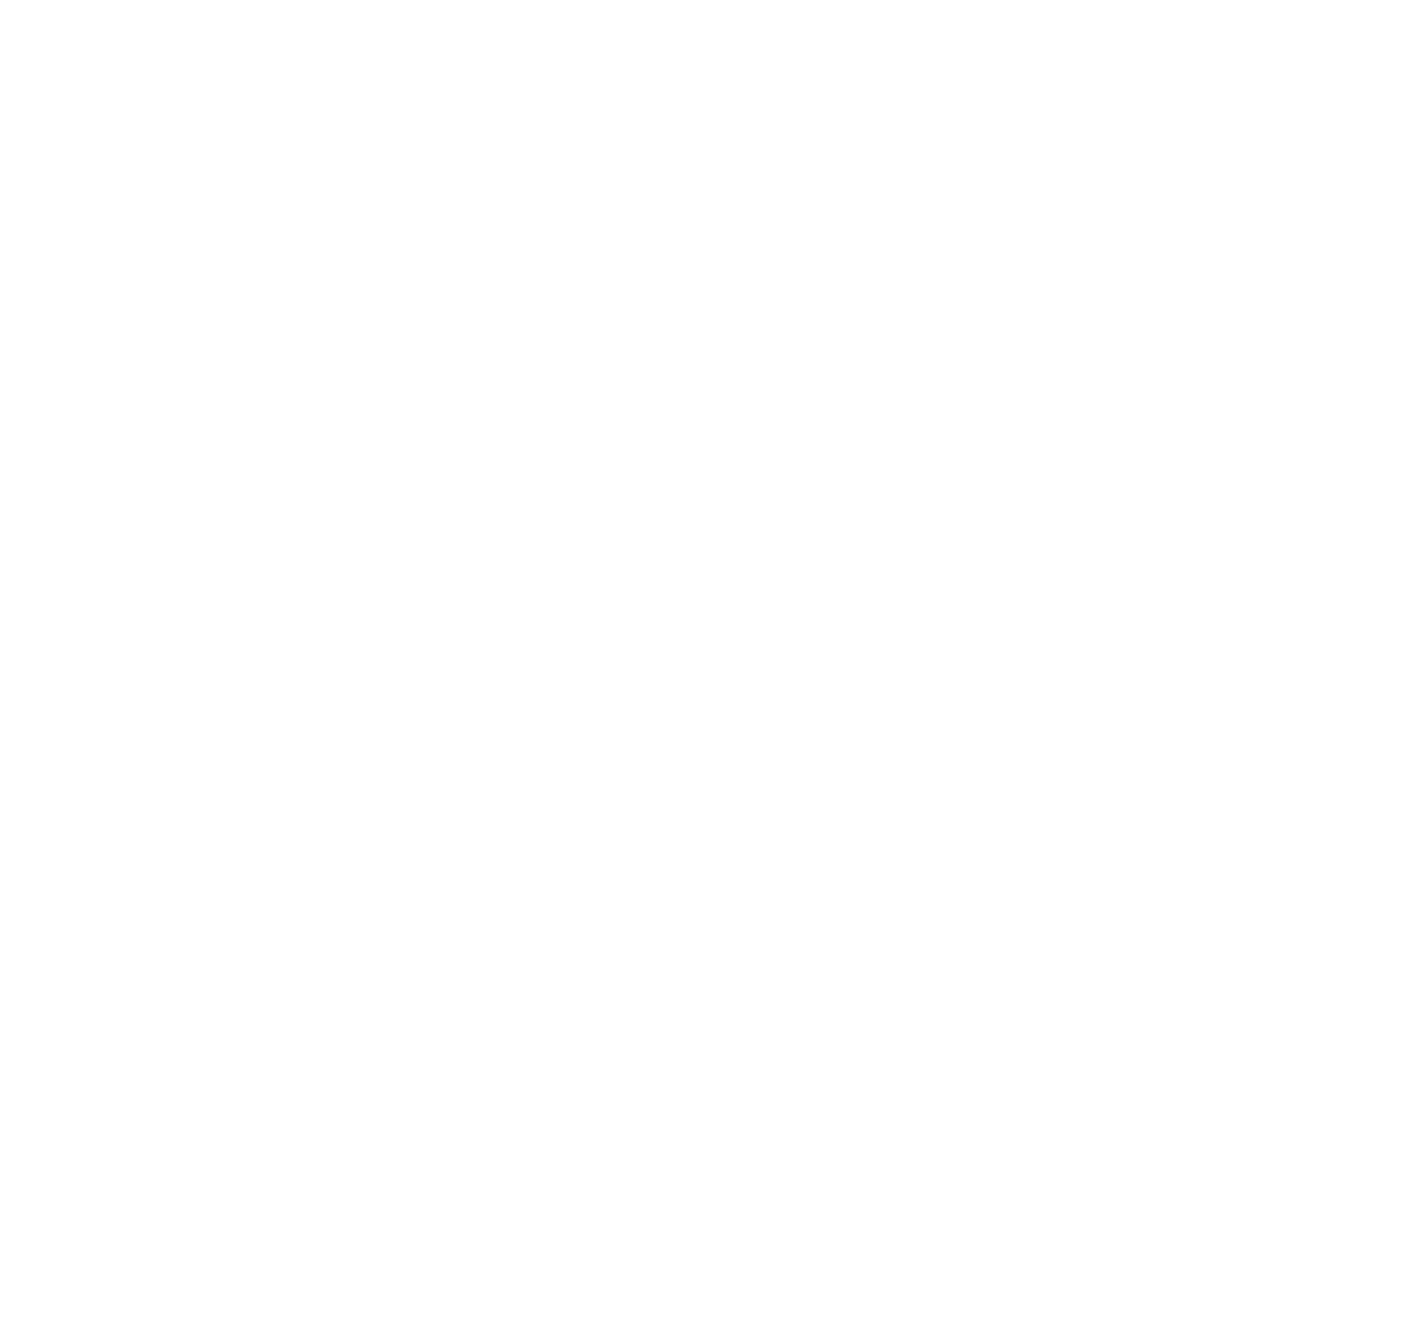
\includegraphics[width=\textwidth]{img/intro-0}}
        \only<2>{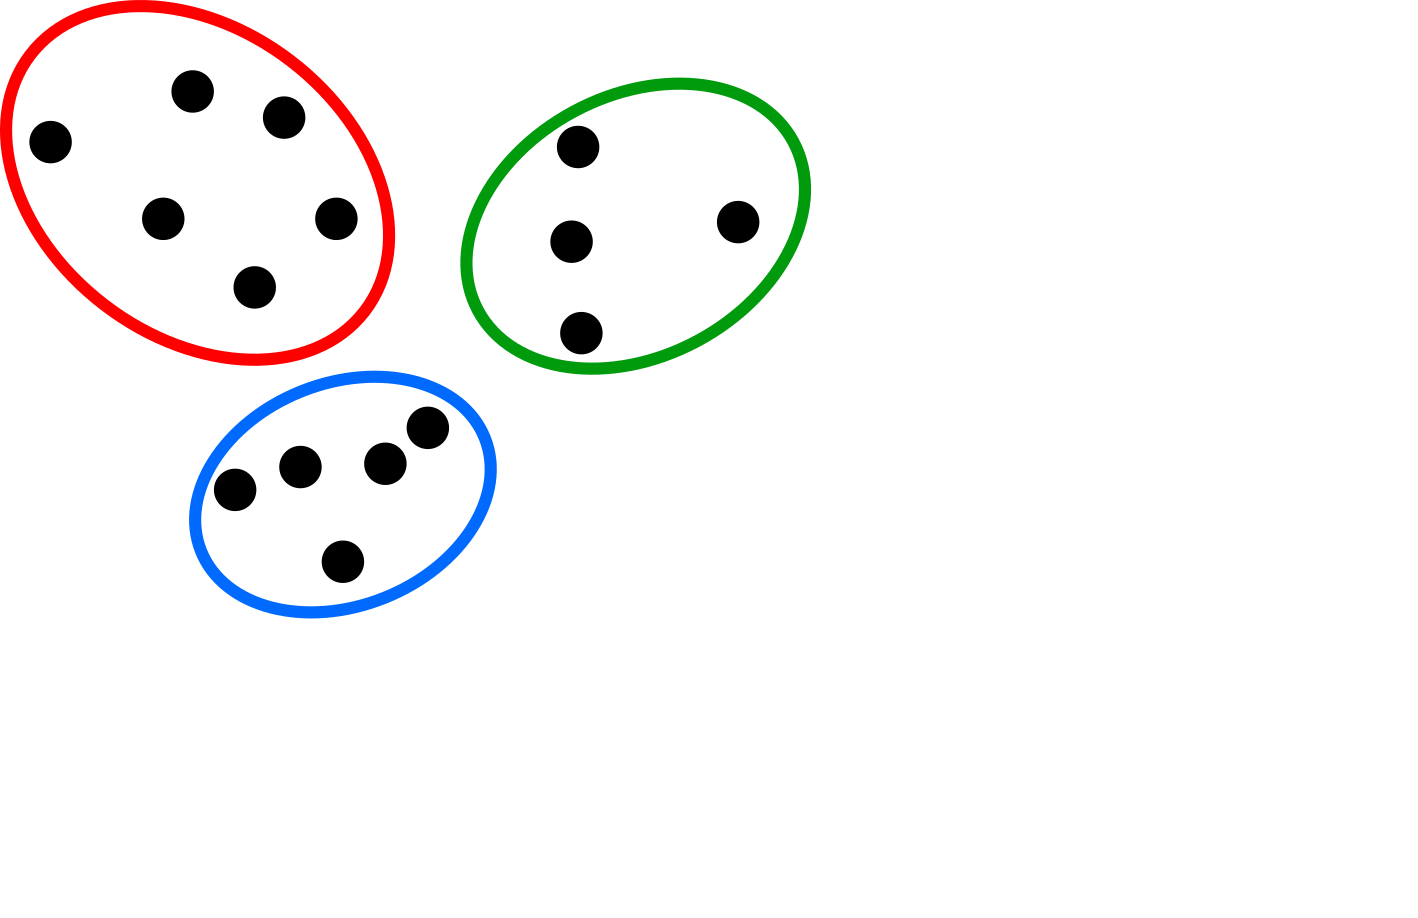
\includegraphics[width=\textwidth]{img/intro-1}}
        \only<3>{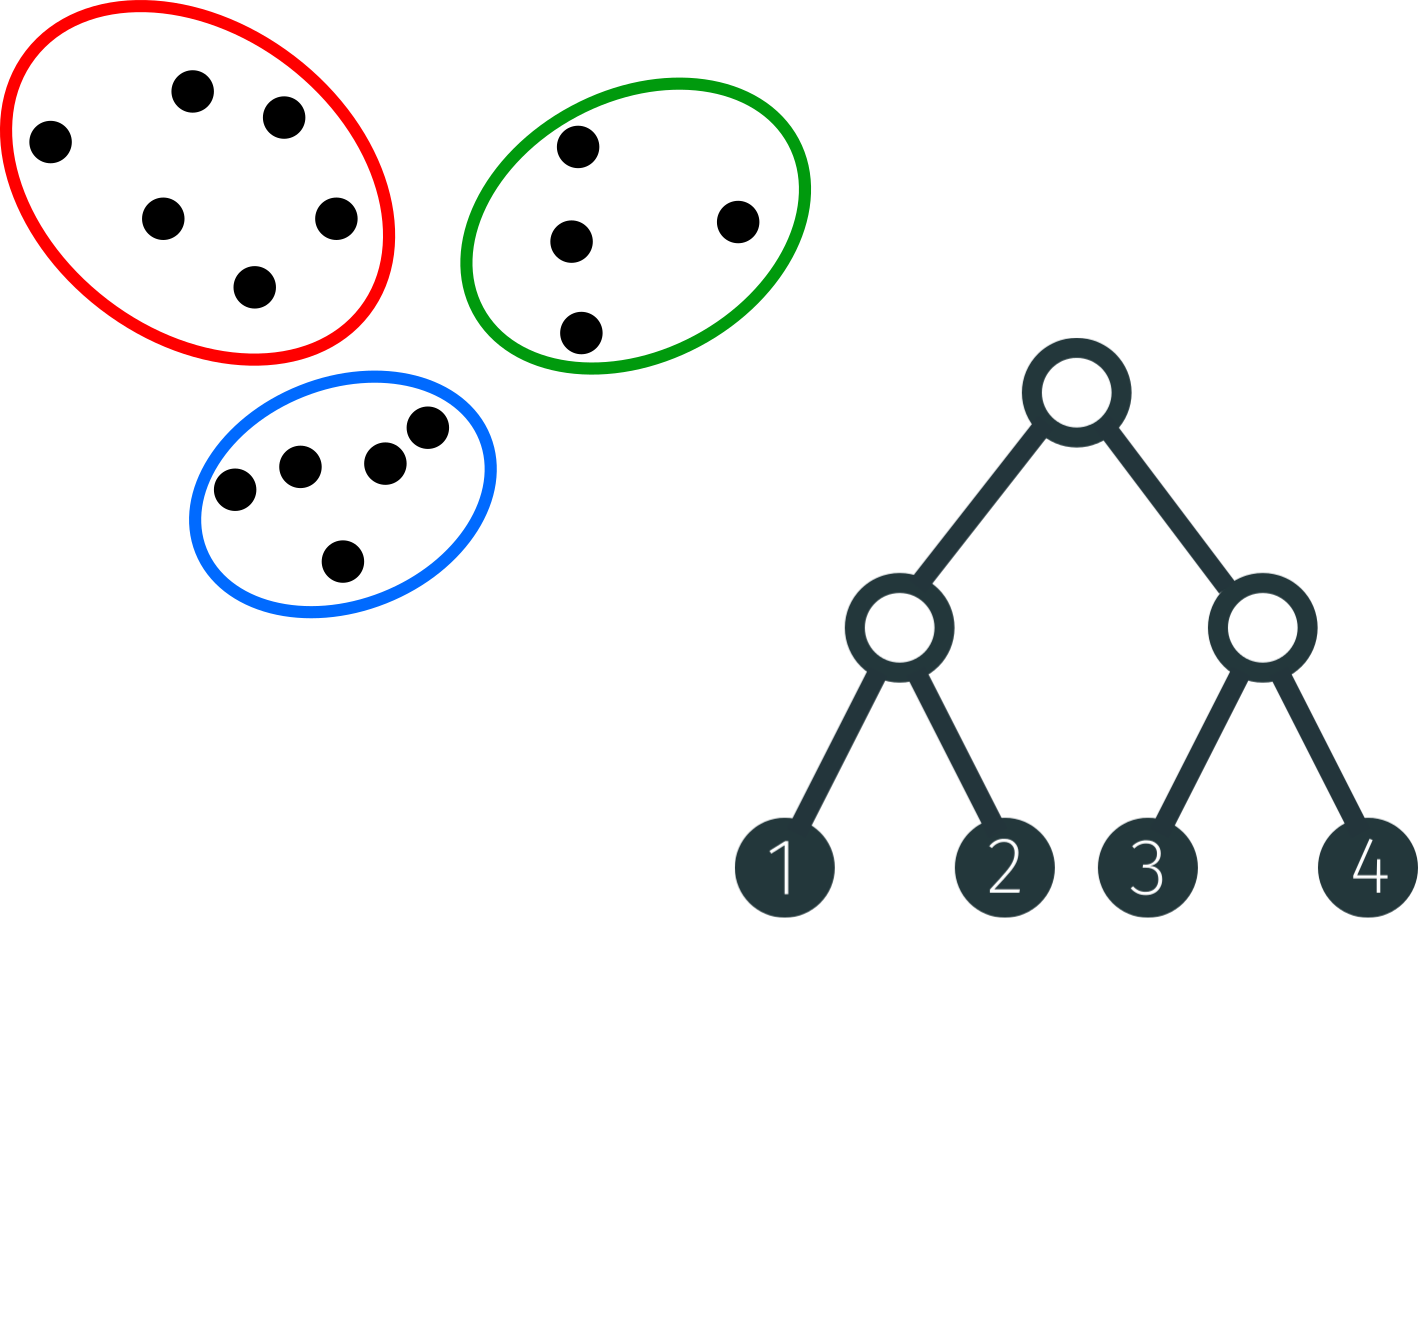
\includegraphics[width=\textwidth]{img/intro-2}}
        \only<4->{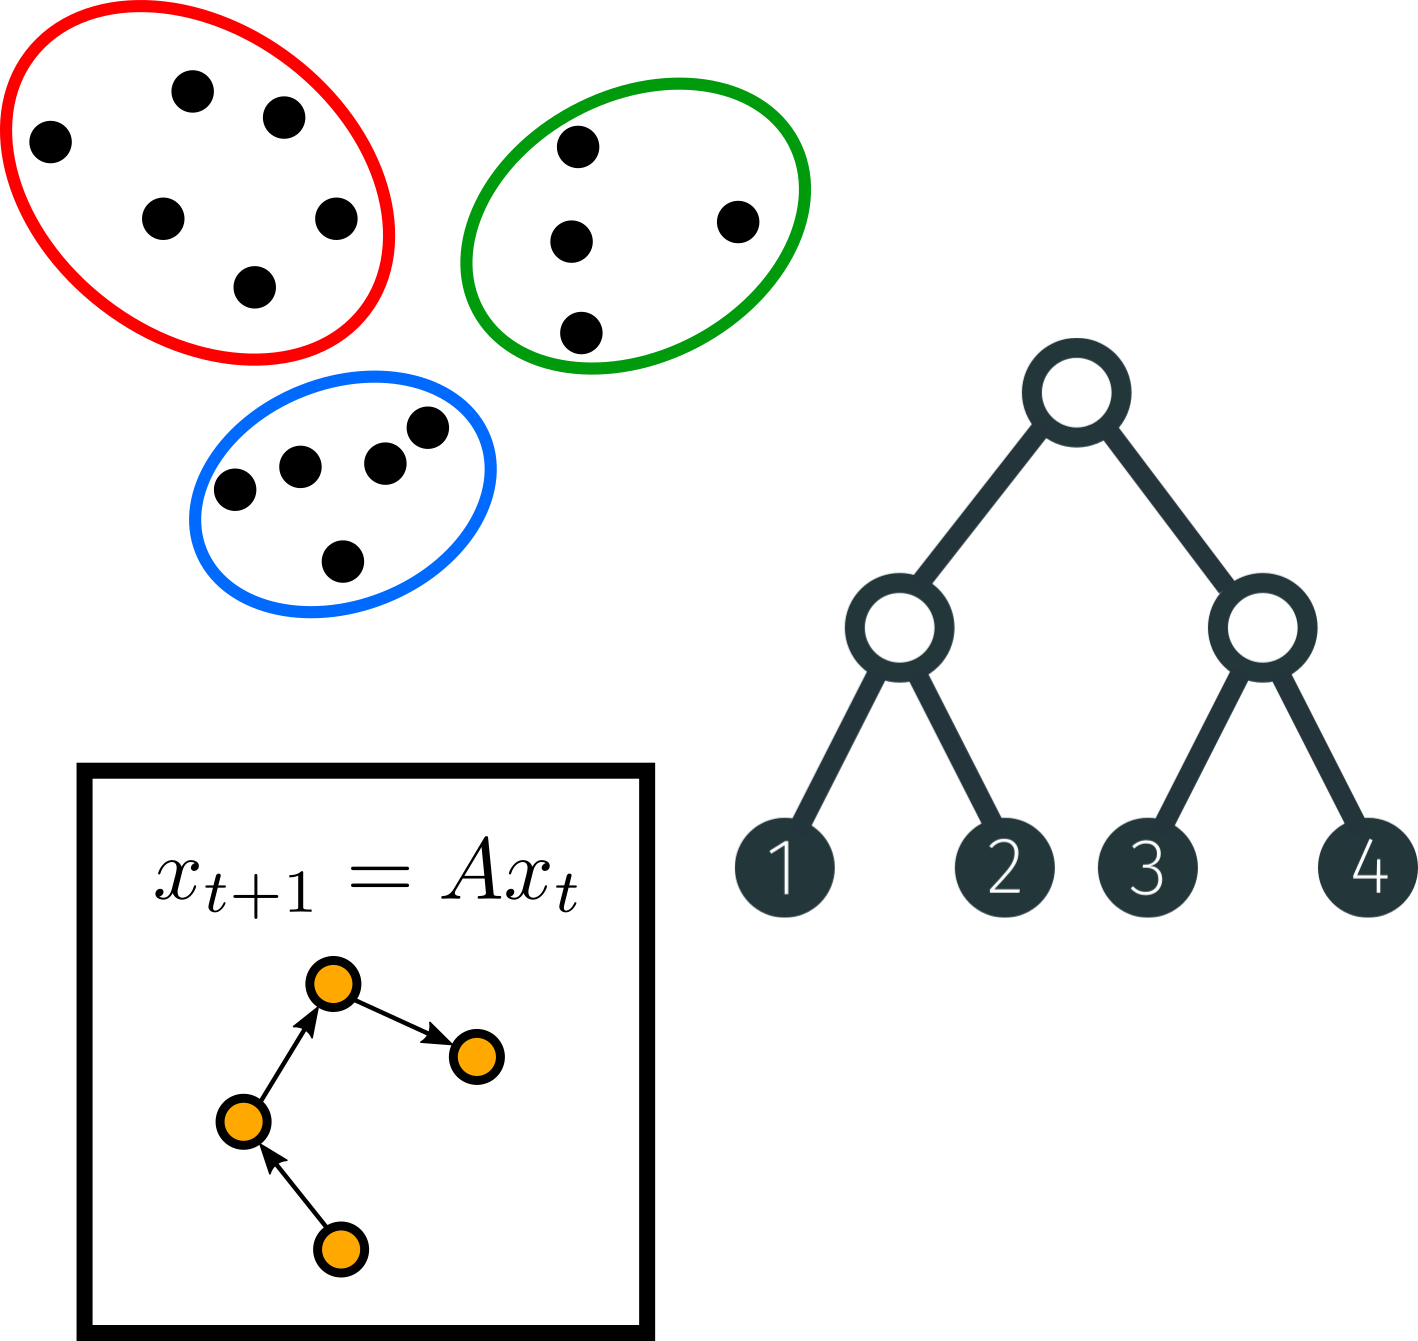
\includegraphics[width=\textwidth]{img/intro-3}}
        \end{center}
      \end{overlayarea}
    \end{column}
    \begin{column}{0.5\textwidth}
      \begin{overlayarea}{\textwidth}{5cm}
        \centering
        \Large \textbf{Embedding} \\ \vspace{10pt}
        \only<5->{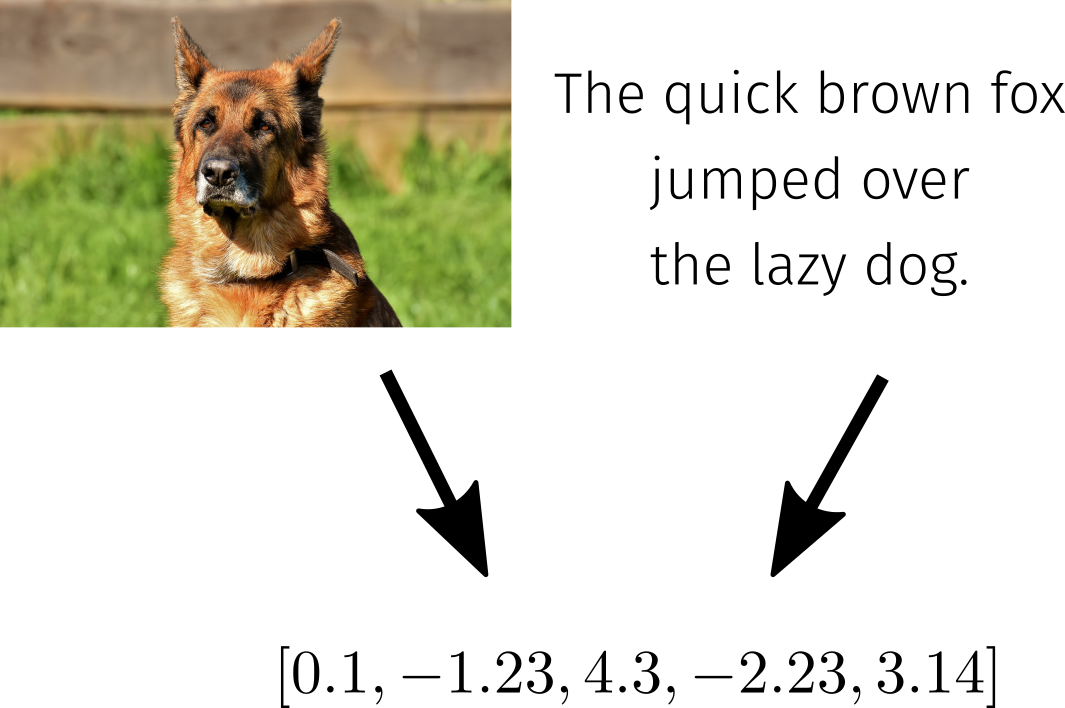
\includegraphics[width=\textwidth]{img/intro-right-1}}
      \end{overlayarea}
    \end{column}
  \end{columns}
\end{frame}

\begin{frame}{Bayesian unsupervised learning}
  \centering
  \begin{columns}[T]
    \begin{column}{0.5\textwidth}
      \begin{overlayarea}{\textwidth}{7cm}
        \begin{center}
          \Large \textbf{Structure}\\ \vspace{10pt}
          \multiinclude[<+>][format=png, start=1]{img/bayesian-intro-left}
        \end{center}
      \end{overlayarea}
    \end{column}
    \begin{column}{0.5\textwidth}
      \begin{overlayarea}{\textwidth}{5cm}
        \pause
        \centering
        \Large \textbf{Embedding} \\ \vspace{60pt}
        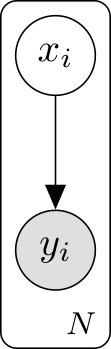
\includegraphics[]{img/bayesian-intro-right-1}
      \end{overlayarea}
    \end{column}
  \end{columns}
\end{frame}

\begin{frame}{Research overview}
  \centering
  \multiinclude[<+>][format=png, graphics={width=0.8\textwidth}]{img/overview}
\end{frame}

\section{Structure learning}

\begin{frame}{Structure learning}
  \centering
  What is structure learning?

  \pause
  \centering
  \begin{figure}
    \centering
    \pause
    \begin{subfigure}[t]{0.27\textwidth}
        \centering
        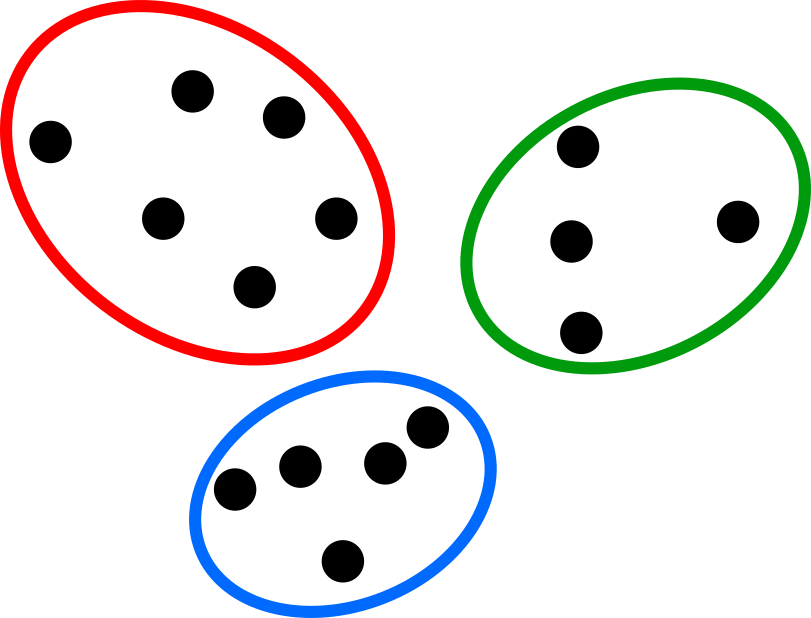
\includegraphics[width=\textwidth]{img/clustering}
    \end{subfigure}
    \pause
    \hfill
    \begin{subfigure}[t]{0.27\textwidth}
        \centering
        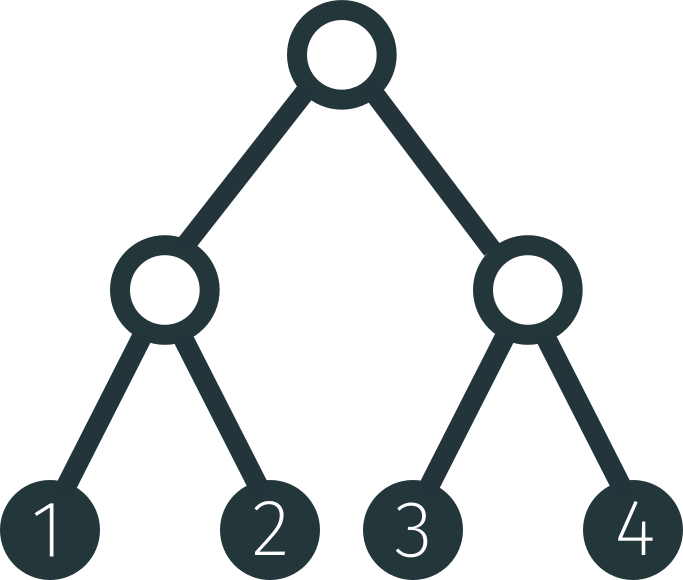
\includegraphics[width=\textwidth]{img/tree-1234-balanced}
    \end{subfigure}
    \pause
    \hfill
    \begin{subfigure}[t]{0.27\textwidth}
        \centering
        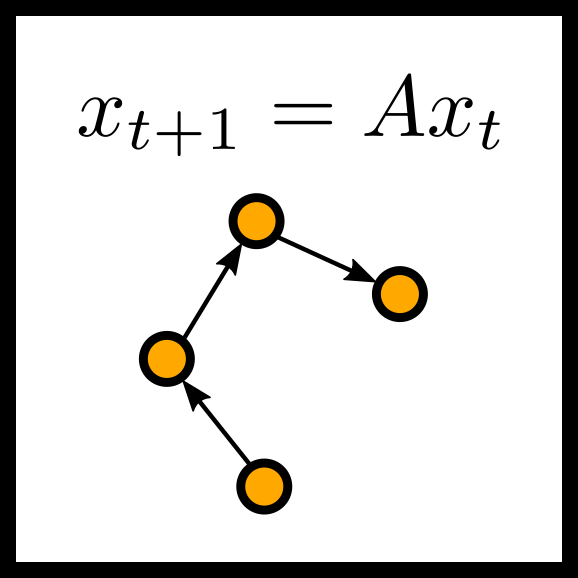
\includegraphics[width=\textwidth]{img/lds}
    \end{subfigure}
  \end{figure}
  \pause
  Structure learning seeks out patterns in data that has intuitive meaning to us

\end{frame}

\begin{frame}{Challenge: ambiguity}
  \centering
  \only<1-5>{Consider the clustering scenario.}
  
  \only<6>{A Bayesian approach models this ambiguity}
  
  \multiinclude[<+->][format=png, start=0, end=4]{img/ambiguous-bayes}

\end{frame}

\begin{frame}{Can we do better?}
  \centering

  \only<-3>{
    \vspace{20pt}
    \multiinclude[<+-3>][format=png]{img/cluster-interaction}
    \vspace{20pt}
  }

  \only<4>{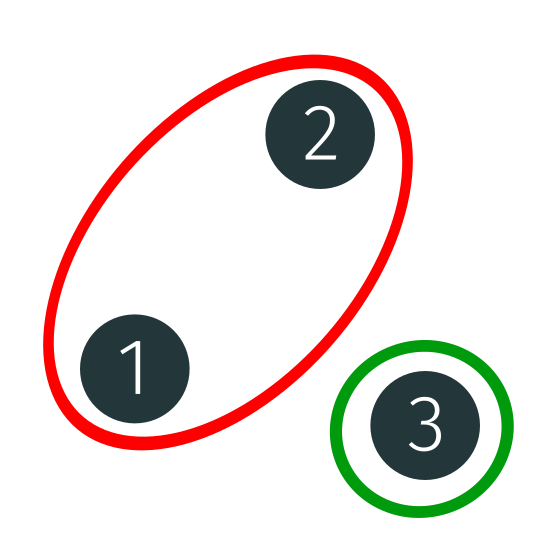
\includegraphics{img/ambiguous-cluster3-2}}

  \onslide<3-4>{User provides constraint $1$ must link with $2$.}

\end{frame}

\begin{frame}{Interactive structure learning}

  \multiinclude[<+>][graphics={width=\textwidth}, format=png, start=1]{img/structure-interaction}

  \onslide<2->{Algorithm provides a structure $S$}
  \onslide<3->{and human provides a constraint $c$}

\end{frame}

\begin{frame}{Bayesian interactive structure learning}
  \centering
  How are these problems framed in the Bayesian setting?

  \pause
  \vspace{10pt}

  \only<2>{\includegraphics{tikz/structure}}

  \only<3>{\includegraphics{tikz/interactive-structure}}

  \onslide<2>{\textbf{Structure learning:} We are interested in $p(S | \bm{y})$}

  \onslide<3>{\textbf{Interactive structure learning:} We are interested in $p(S | \bm{y}, c)$}

\end{frame}

\begin{frame}{Work in Bayesian interactive structure learning}
  \begin{itemize}
    \item Constrained clustering - \cite{Wagstaff2000ClusteringConstraints, NelsonRevisitingConstraints, ShentalComputingConstraints, LangeLearningData} \\
    \pause
    \begin{center}
    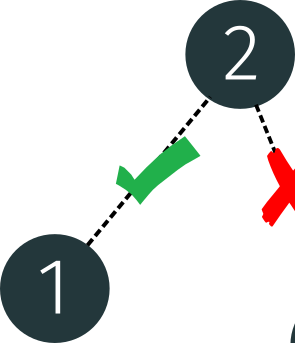
\includegraphics[]{img/must-link} \hspace{20pt} 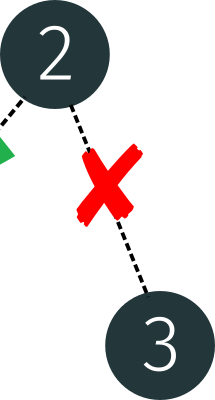
\includegraphics[]{img/mustnot-link}
    \end{center}
    \pause
    \item Constrained Bayesian hierarchical clustering - \cite{Vikram2016} \pause $\begin{array}{l}
\includegraphics{img/overview-digit-1}\end{array}$
  \end{itemize}
\end{frame}

\begin{frame}{Interactive hierarchical clustering}
  \begin{center}
    \includegraphics<1>[width=\textwidth]{img/interaction-0}
    \includegraphics<2>[width=\textwidth]{img/interaction-1}
    \includegraphics<3>[width=\textwidth]{img/interaction-2}
    \includegraphics<4->[width=\textwidth]{img/interaction-3}
  \end{center}
  \begin{itemize}
    \item<4-> User provides a \alert{triplet}. $a$ and $b$
  should be in a subtree together without $c$.
    \item<5-> We show the user the induced tree on a subset of the data $T|_S$.
  \end{itemize}
\end{frame}

\begin{frame}{Bayesian hierarchical clustering}
  We desire a probability distribution over all possible
  trees that explain the data.

    \pause
  \begin{center}
    %\includegraphics<2>[width=0.7\textwidth]{img/3-cluster-distribution.png}
    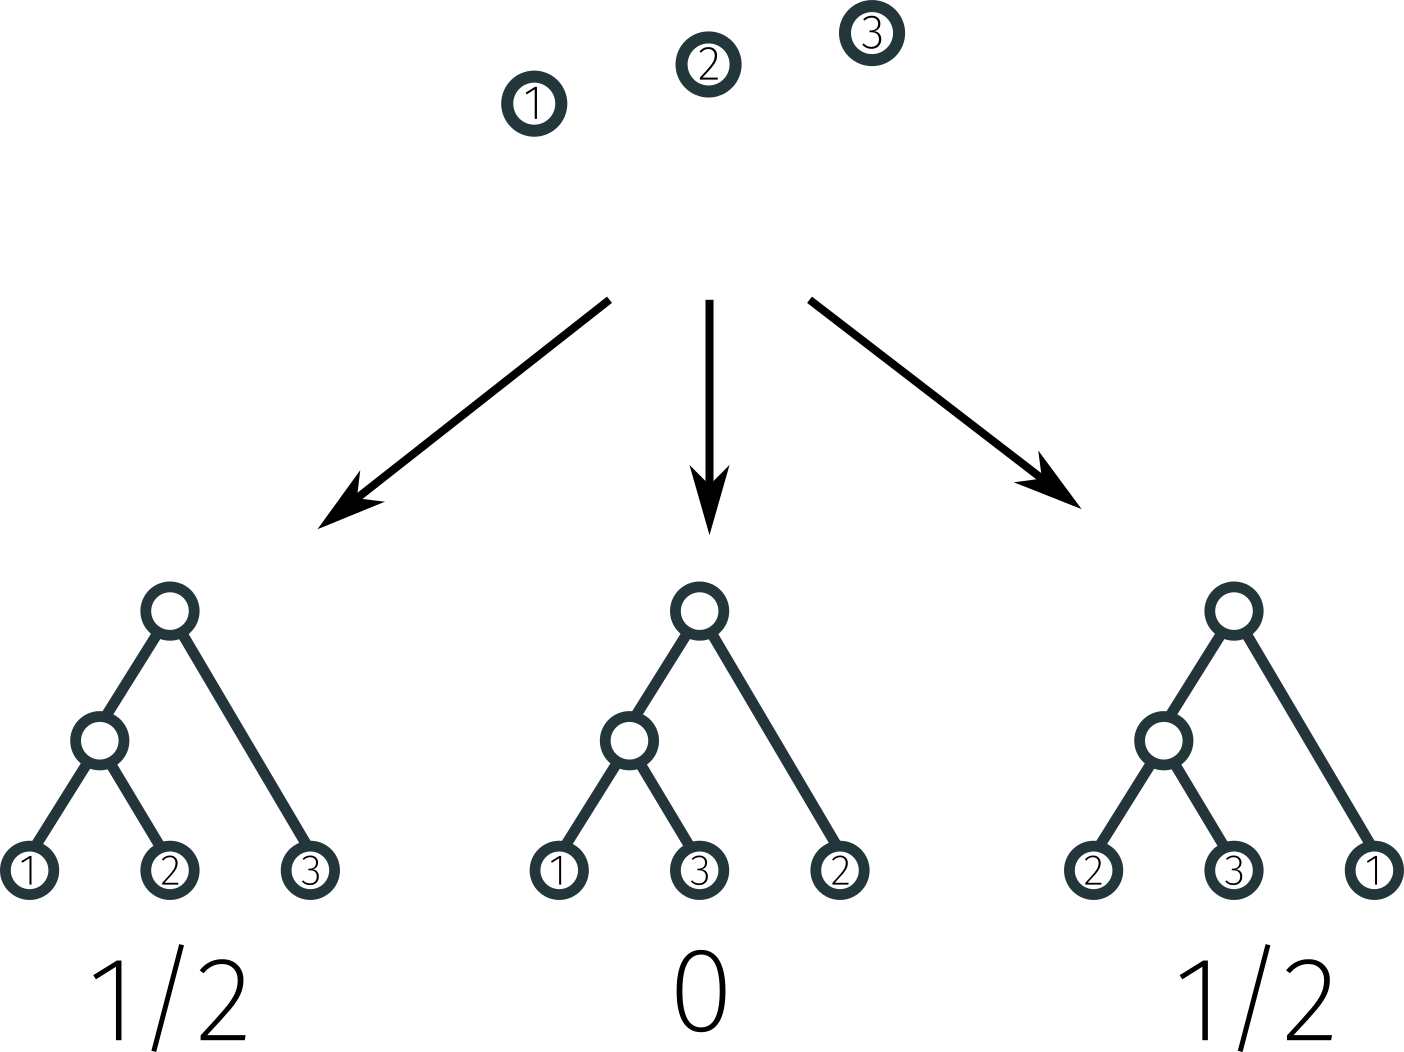
\includegraphics[width=0.7\textwidth]{img/3-cluster-linear-distribution.png}
  \end{center}
\end{frame}

\begin{frame}{Bayesian hierarchical clustering: generative process}
  Define a generative model for the data.
  \begin{center}
  $\begin{array}{l}\includegraphics{tikz/tmc}\end{array}$ 
  \end{center}
  
  \begin{itemize}
    \pause
    \item Prior distribution $p(\tau)$, (Dirichlet diffusion tree,
      Kingman's coalescent, Time-marginalized coalescent)
    \pause
    \item Likelihood model $p(\bm{x} | \tau)$, (Brownian motion,
      Dirichlet-multinomial diffusion)
  \end{itemize}

  \begin{center}
    \includegraphics<2-3>[width=0.6\textwidth]{img/tree-data-0}
    \includegraphics<4>[width=0.6\textwidth]{img/tree-data-1}
  \end{center}

\end{frame}

\begin{frame}{Inference in BHC}
  We are interested in the posterior distribution
  $p(\tau | \bm{x})$, which we compute
  via MCMC methods like Metropolis-Hastings.
  
  \pause

  A popular local search step is \alert{subtree-prune
  and regraft} (SPR).

  \begin{center}
    \multiinclude[<+>][format=png, graphics={width=\textwidth}, start=1]{img/spr}
  \end{center}

\end{frame}

\begin{frame}{Incorporating triplet feedback}

  Recall the interaction model.

  \begin{center}
    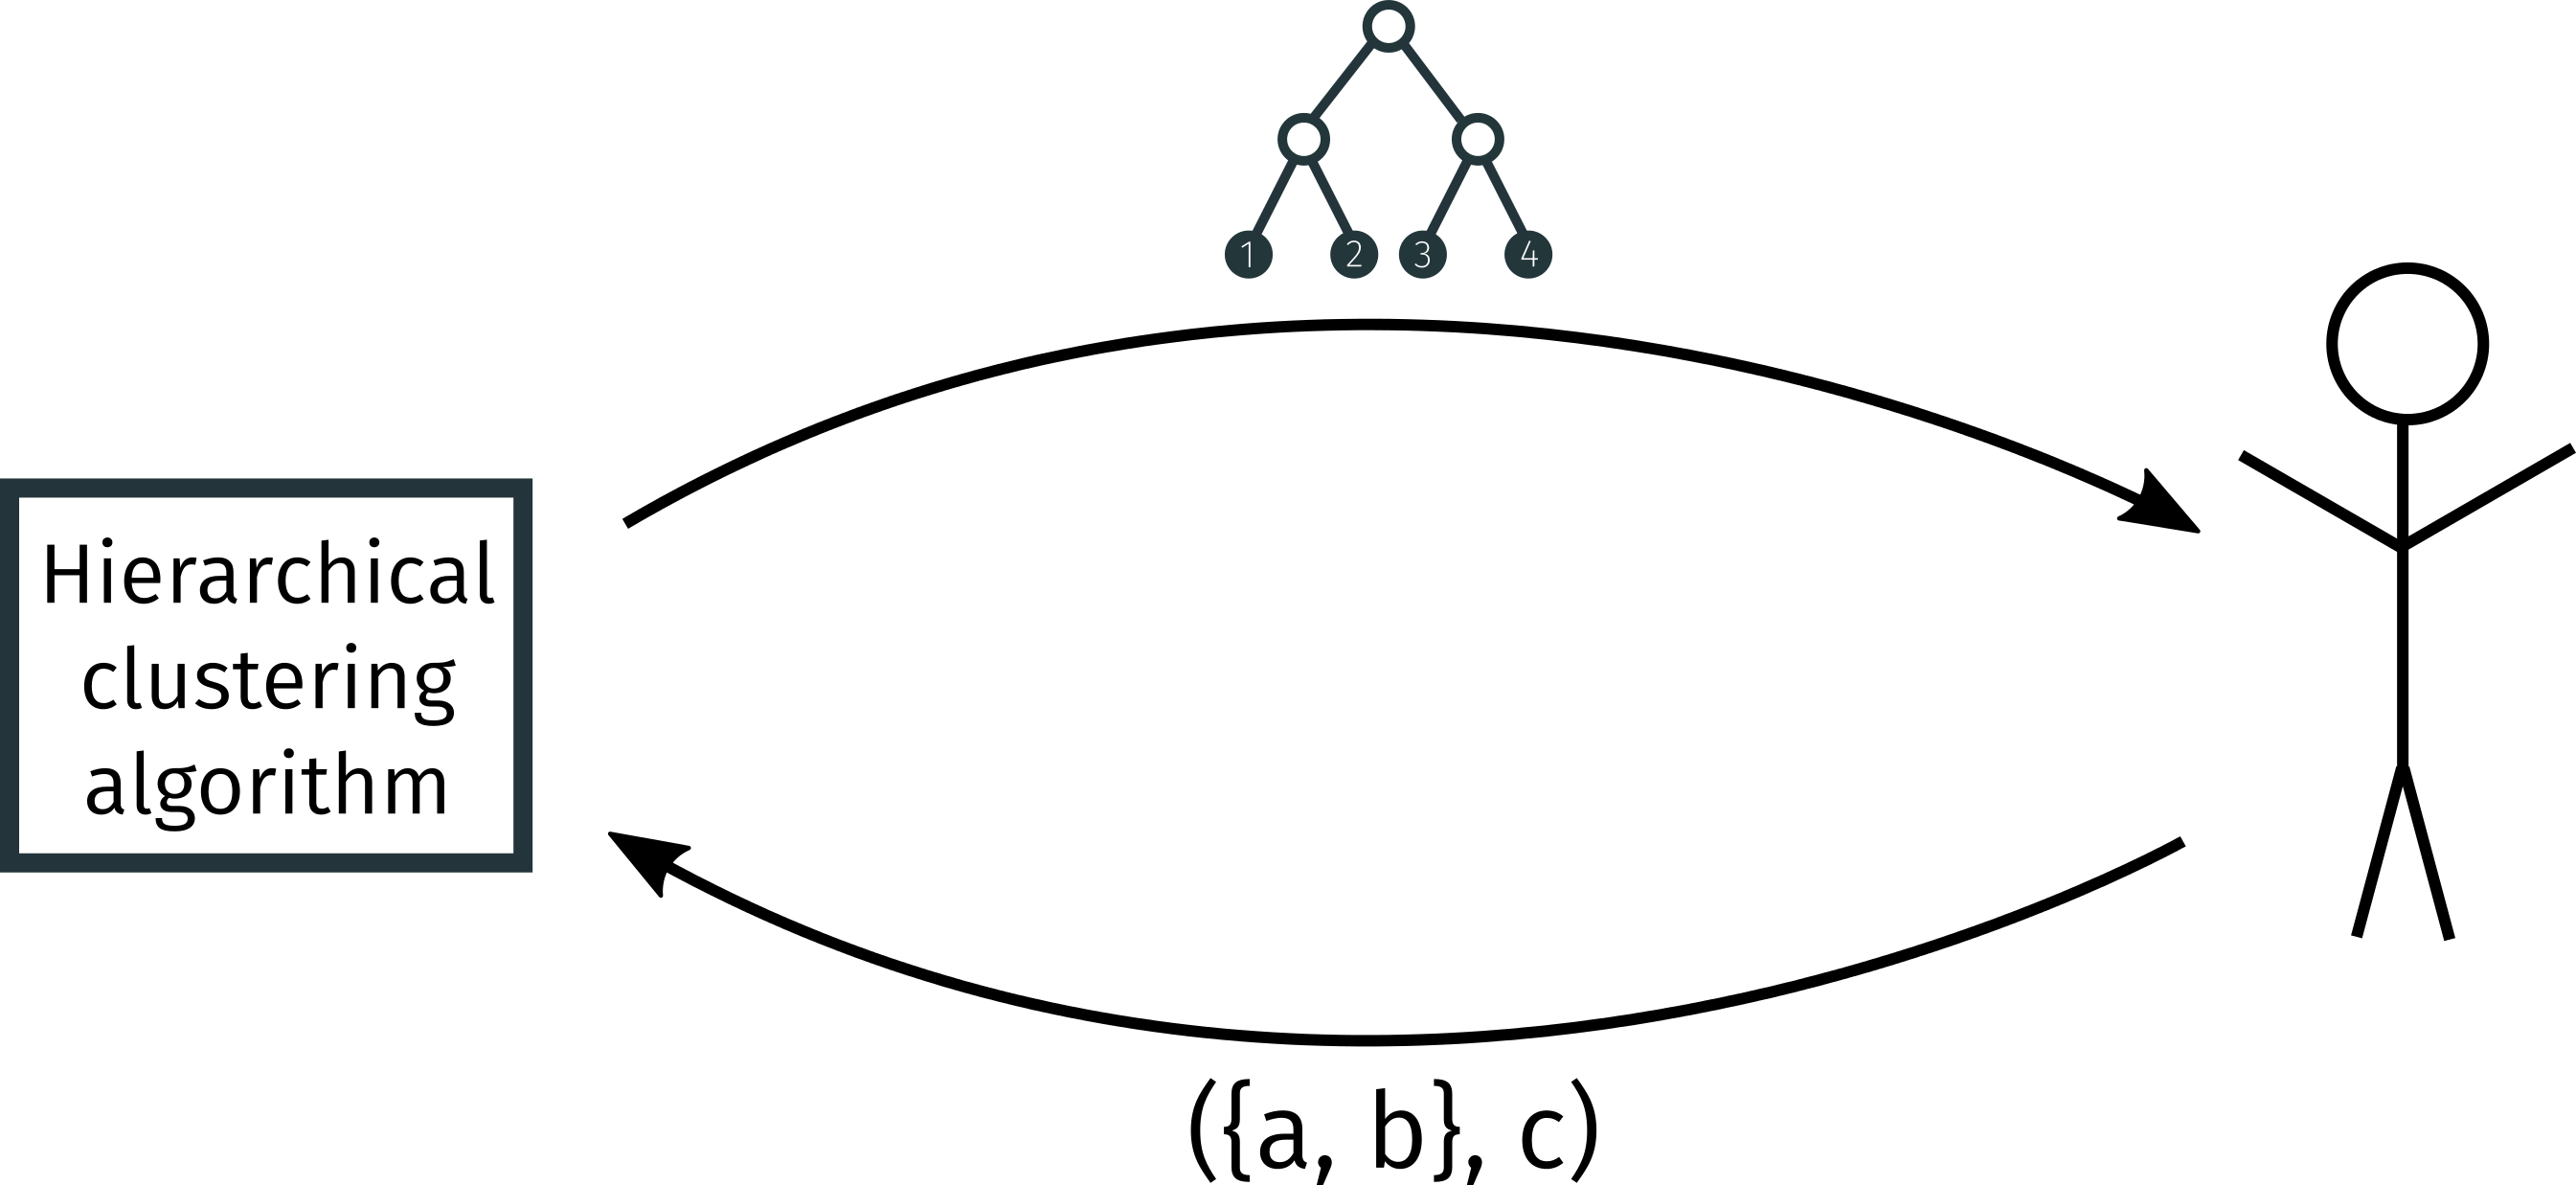
\includegraphics[width=0.7\textwidth]{img/interaction-3}
  \end{center}
  \pause

  \textbf{Idea:}  enforce triplet constraints with
  modified SPR move

  \pause

  \begin{center}
    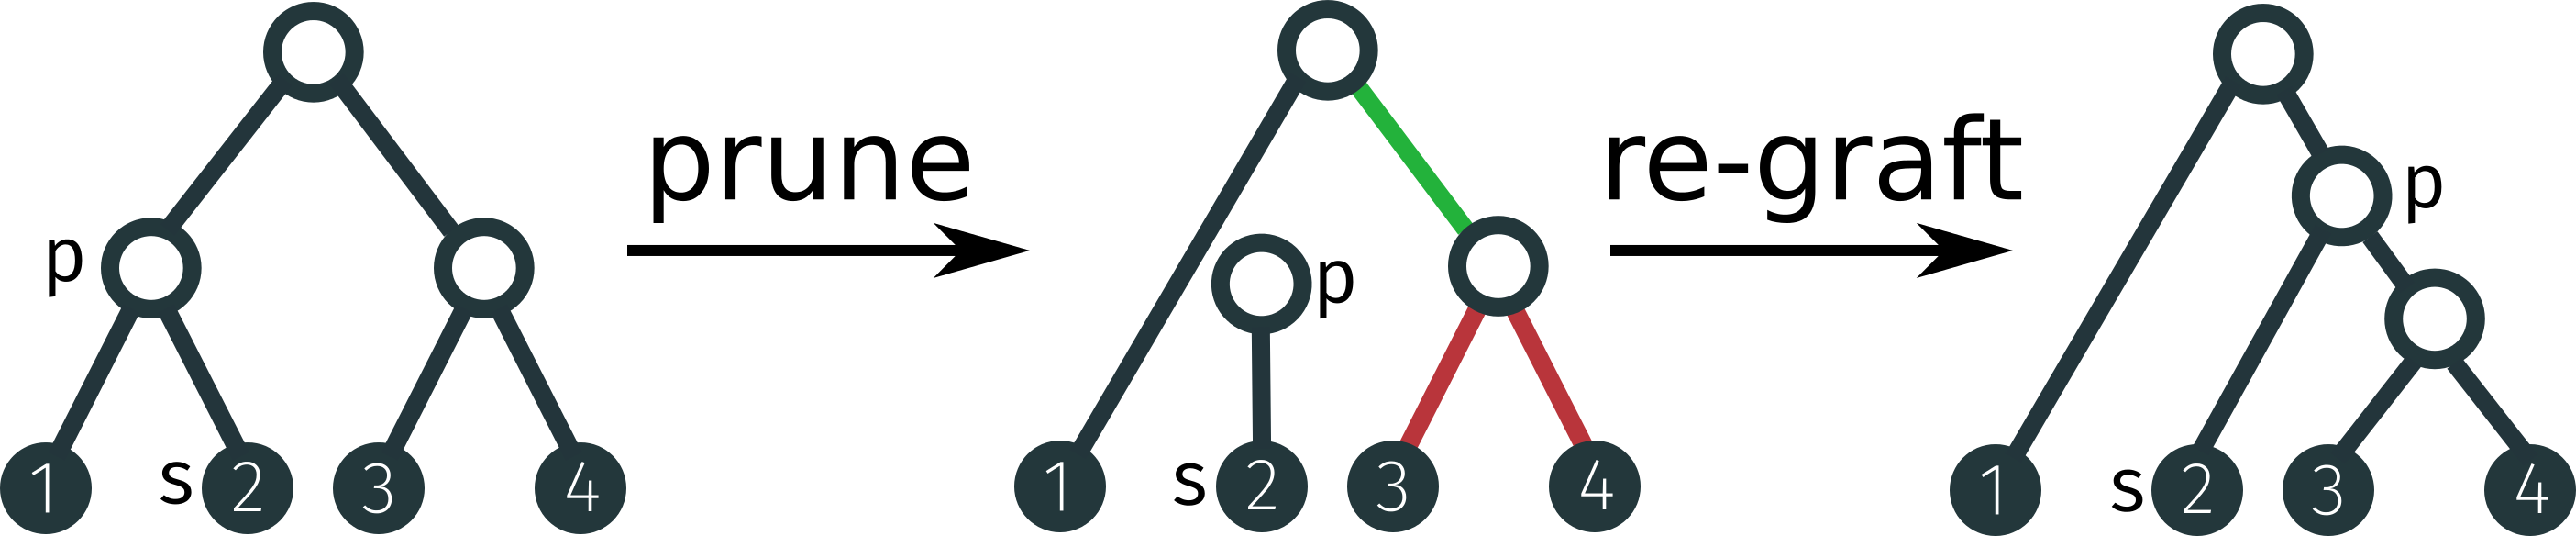
\includegraphics[width=\textwidth]{img/cspr-animation}
  \end{center}
\end{frame}

\begin{frame}{Results}
  \centering
  \vspace{10pt}
  \begin{figure}
  \frame{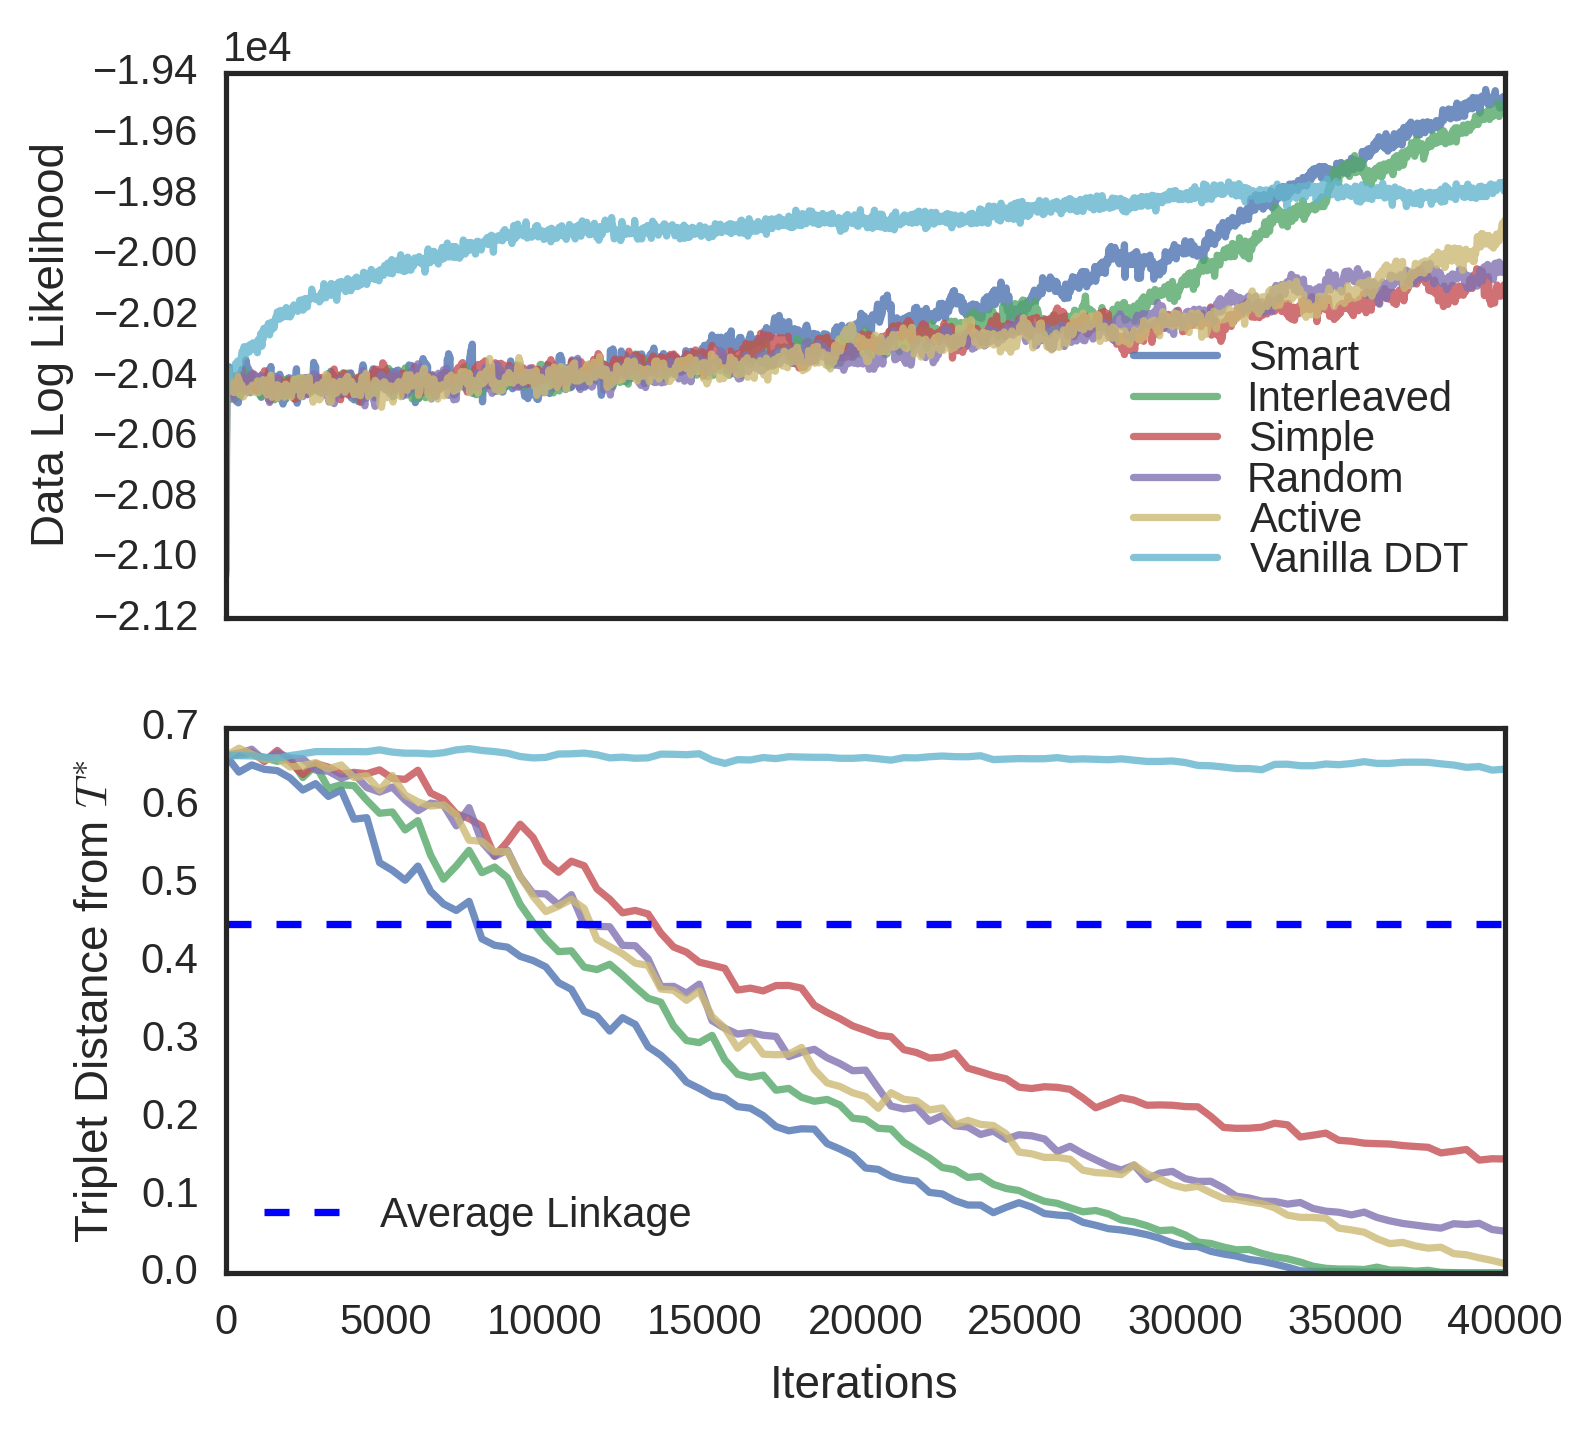
\includegraphics[width=0.7\textwidth]{img/trees/MNIST-result}}
  \caption*{Results of interactive Bayesian hierarchical clustering on MNIST}
  \end{figure}
\end{frame}

\begin{frame}{Overview}
  \centering
  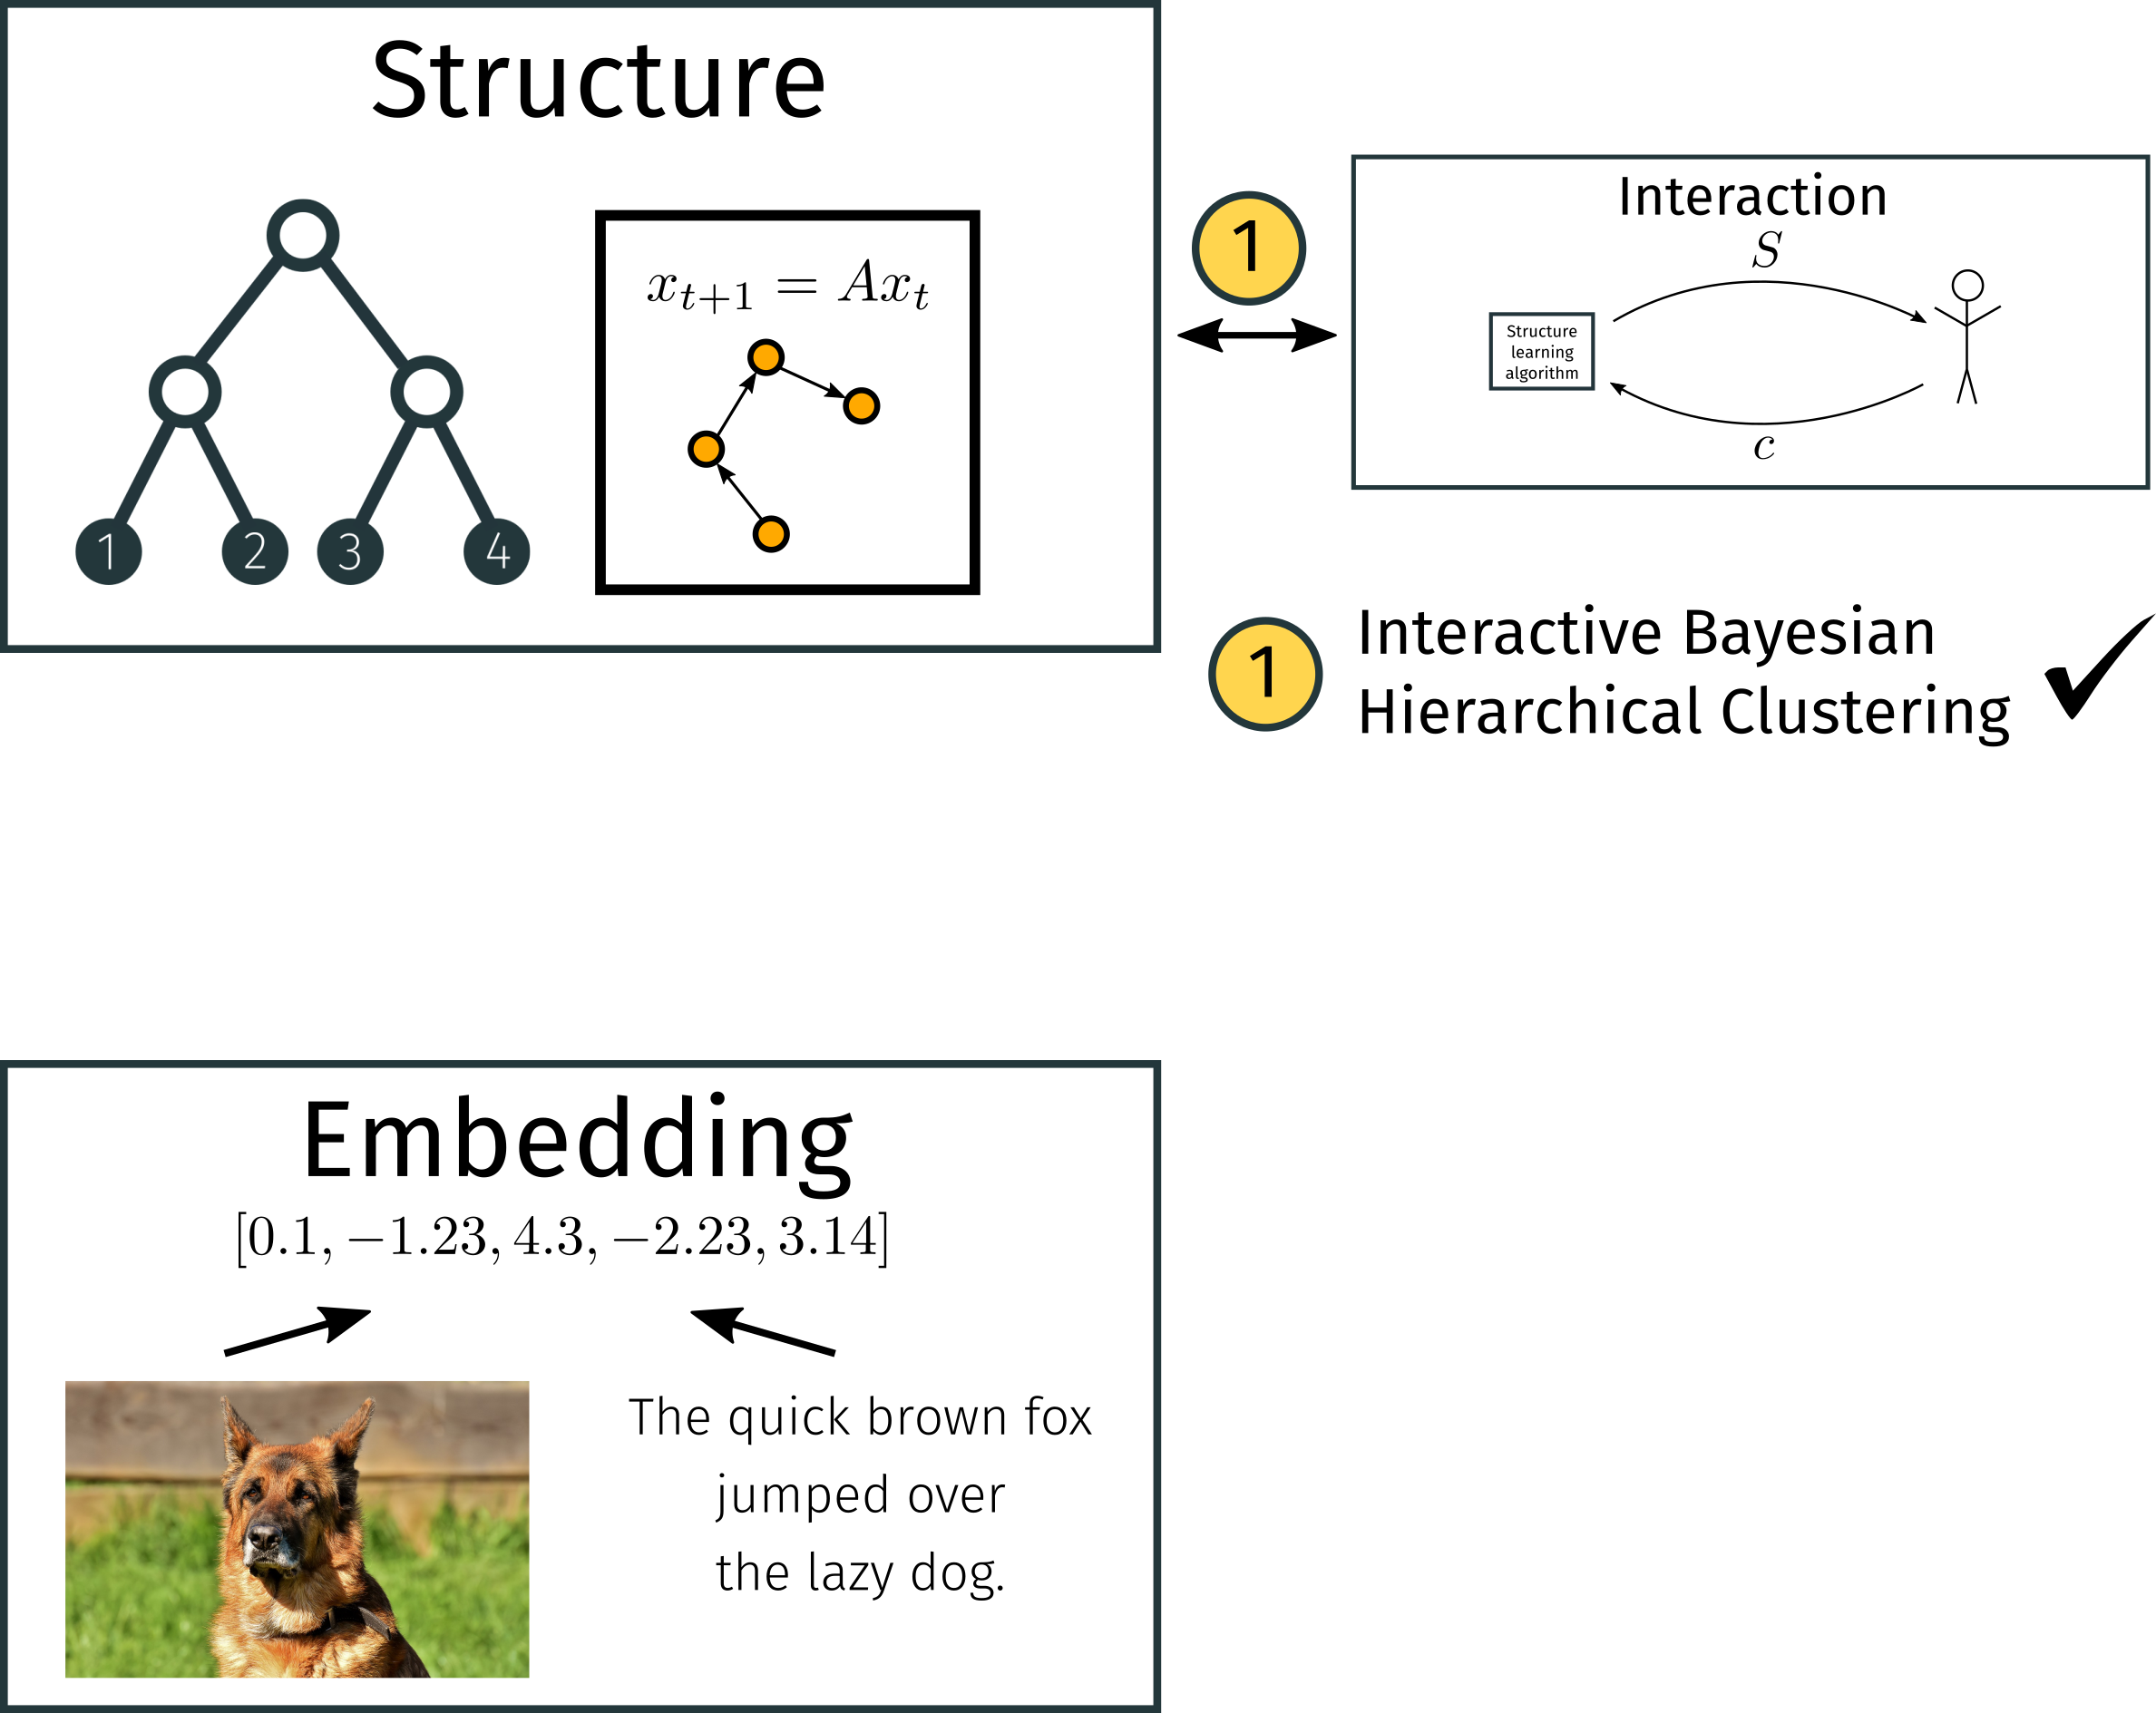
\includegraphics[width=0.8\textwidth]{img/overview-1}
\end{frame}

\section{Embedding learning (background)}

\iffalse
\begin{frame}{Bayesian embedding learning}
  \centering
  What's the difference between embedding and structure learning?
  \pause
  \begin{center}
    \begin{columns}
      \begin{column}{0.3\textwidth}
        \includegraphics{tikz/structure}
      \end{column}
    \pause
      \begin{column}{0.3\textwidth}
        \includegraphics{tikz/vae}
      \end{column}
    \end{columns}
  \end{center}
\end{frame}
\fi

\begin{frame}{Variational autoencoder}
  The VAE is a generative model for data.
  \begin{align*}
    x_i &\sim  \N(0, I) \\
    y_i &\sim  \N(\mu_\gamma(x_i), \Sigma_\gamma(x_i))
  \end{align*}
  where $\mu_\gamma$ and $\Sigma_\gamma$ are neural networks parameterized by $\gamma$.

  \pause
  \centering
  \includegraphics{tikz/vae}
  \pause
   
  How do we do inference?
  \alert<+>{Variational inference}
\end{frame}

\begin{frame}{Variational inference at a high level}
  For models where sampling is too slow,
  \textbf{variational inference}
  is a viable approach.

  \pause
    Consider a latent variable model with latent variable 
    $x$ and observation $y$. Our desired
    posterior is $p(x | y)$.

    \pause
    \textbf{Strategy}: convert inference into optimization
    \begin{itemize}
        \pause
      \item Instantiate \emph{variational distribution} $q_\phi(x)$
        where $\phi$ are free parameters
        \pause
      \item Define objective $\elbo[q_\phi(x)]$.
        \pause
      \item Maximize objective $\phi^* = \argmax_\phi \elbo[q_\phi(x)]$
    \end{itemize}
    \pause
    If $q_\phi(x)$ is sufficiently expressive,
    it can approximate $p(x | y)$ quite well.
\end{frame}

\begin{frame}{Evidence lower bound}
  This objective is called the \alert{evidence lower bound} (ELBO).
  
  \pause
  
  \begin{align*}
    \elbo[q(x)] &\triangleq \E_{q(x)}\left[\log\frac{p(y, x)}{q(x)}\right]
  \end{align*}

  It has a unique relationship to the KL divergence $\KL(q(x)\|p(x|y))$.

  We can rewrite the KL divergence as
  \begin{align*}
    \KL(q(x)\|p(x|y)) &= \int q(x)\log\frac{q(x)}{p(x | y)}dx \\
              &= \log p(y) - \E_{q(x)}\left[\log\frac{p(y, x)}{q(x)}\right]
  \end{align*}
  
\end{frame}

\begin{frame}{Variational autoencoder}
  \textbf{Basic strategy:} gradient-based variational inference

  \pause

  \begin{center}
      \begin{framed}
       Pick $q_\phi(x | y)$ (can be conditional) to be a \emph{neural network}
          parameterized by $\phi$
      \end{framed}
  \end{center}

  \pause
  Let $r_\phi(y)$ be a neural network (with weights $\phi$)
  that outputs the parameters to a distribution, for example Gaussian.
  \begin{align*}
    q_\phi(x | y) = \N(r_\phi(y))
  \end{align*}

  \pause
  Goal: learn the weights for the two neural networks $(\mu_\gamma(x), \Sigma_\gamma(x))$ and $r_\phi(y)$
  via SGD on the ELBO.
  \pause
  \begin{align*}
    \elbo[q_\phi(x | y)] &= \E_{q_\phi(x | y)}\left[\log\frac{p(y, x)}{q_\phi(x | y)}\right]
  \end{align*}
\end{frame}

\begin{frame}{Sidebar: Monte-Carlo ELBO}
  We can't compute the ELBO because of the expectation w.r.t $q_\phi(x|y)$.
  \begin{align*}
    \elbo[q_\phi(x | y)] &= \E_{q_\phi(x | y)}\left[\log \frac{p(y, x)}{q_\phi(x | y)}\right]
  \end{align*}
  We can sample from $q$ however:
  \begin{align*}
    \hat{\elbo}[q_\phi(x | y)] &\triangleq \frac{1}{L}\sum_{l = 1}^L \log \frac{p(y, x^{(l)})}{q_\phi(x^{(l)} | y)}
  \end{align*}
  Now, we can compute gradients.
  \begin{align*}
    \gamma^{(t + 1)} &\leftarrow \gamma^t + \rho \nabla_\gamma \hat{\elbo} \\
    \phi^{(t + 1)} &\leftarrow \phi^t + \rho \nabla_\phi \hat{\elbo} \\
  \end{align*}
\end{frame}

\section{Structured embedding learning}

\begin{frame}{Structured embedding models}
  \begin{figure}
    \centering
    \pause
    \begin{subfigure}[t]{0.27\textwidth}
        \centering
        \includegraphics{tikz/lgmm}
        \caption*{Latent GMM}
    \end{subfigure}
    \pause
    \hfill
    \begin{subfigure}[t]{0.27\textwidth}
        \centering
        \includegraphics{tikz/ltmc}
        \caption*{Latent hierarchical clustering}
    \end{subfigure}
    \pause
    \hfill
    \begin{subfigure}[t]{0.27\textwidth}
        \centering
        \includegraphics{tikz/llds}
        \caption*{Latent LDS}
    \end{subfigure}
  \end{figure}
\end{frame}

\begin{frame}{Structured variational autoencoder}
  SVAE - \cite{Johnson2016}
  \centering
  \begin{columns}
    \begin{column}{0.3\textwidth}
      \includegraphics{tikz/lgmm}
    \end{column}
    \begin{column}{0.3\textwidth}
      \begin{align*}
        \pi &\sim \textrm{Dirichlet}(\alpha) \\
        \{\mu_k, \Sigma_k\}_{k = 1}^K &\sim \NIW(\Psi, \mu_0, \kappa, \nu) \\
        z_i | \pi &\sim \textrm{Categorical}(\pi) \\
        x_i | z_i, \{\mu_k, \Sigma_k\}_{k = 1}^K \ &\sim \N(\mu_{z_i}, \Sigma_{z_i}) \\
        y_i | x_i &\sim \N(\mu_\gamma(x_i), \Sigma_\gamma(x_i))
      \end{align*}
    \end{column}
  \end{columns}
\end{frame}

\begin{frame}{Why SVAE?}
  \begin{center}
    \begin{figure}
    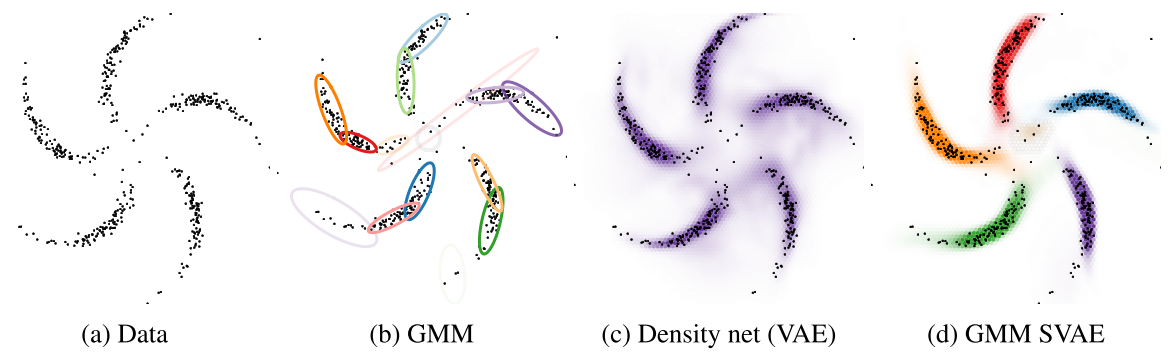
\includegraphics[frame,width=\textwidth]{img/svae-example}
    \caption{\cite{Johnson2016}}
    \end{figure}
  \end{center}

  \pause
  In this scenario, the SVAE enables modeling non-Gaussian cluster shapes.
\end{frame}

\begin{frame}{Structured variational autoencoder}
  \centering
  \begin{columns}
    \begin{column}{0.3\textwidth}
      \includegraphics{tikz/lgmm}
    \end{column}
    \begin{column}{0.3\textwidth}
      \begin{align*}
        \pi &\sim \textrm{Dirichlet}(\alpha) \\
        \{\mu_k, \Sigma_k\}_{k = 1}^K &\sim \NIW(\Psi, \mu_0, \kappa, \nu) \\
        z_i | \pi &\sim \textrm{Categorical}(\pi) \\
        x_i | z_i, \{\mu_k, \Sigma_k\}_{k = 1}^K \ &\sim \N(\mu_{z_i}, \Sigma_{z_i}) \\
        y_i | x_i &\sim \N(\mu_\gamma(x_i), \Sigma_\gamma(x_i))
      \end{align*}
    \end{column}
  \end{columns}
  \pause
  How do we do inference?
\end{frame}

\begin{frame}{What makes inference in these models hard?}
  \begin{figure}
    \centering
    \begin{subfigure}[t]{0.23\textwidth}
        \centering
        \includegraphics{tikz/lgmm}
        \caption*{Latent GMM}
    \end{subfigure}
    \hfill
    \begin{subfigure}[t]{0.23\textwidth}
        \centering
        \includegraphics{tikz/ltmc}
        \caption*{Latent hierarchical clustering}
    \end{subfigure}
    \hfill
    \begin{subfigure}[t]{0.23\textwidth}
        \centering
        \includegraphics{tikz/llds}
        \caption*{Latent LDS}
    \end{subfigure}
  \end{figure}
  \pause
  \centering
  All of these models have a \alert{nonconjugate} edge!
\end{frame}

\begin{frame}[standout]
  \centering
  Can we generalize using neural networks as a tool
  for approximate inference?
\end{frame}

\begin{frame}{Mean-field variational inference}
  \centering
  What happens if the model is simple (conjugate-exponential)? 
  
  \pause Mean-field variational inference
  
  \begin{columns}
    \begin{column}{0.3\textwidth}
      \includegraphics{tikz/gmm}
    \end{column}
    \begin{column}{0.5\textwidth}
        \begin{itemize}
            \item Initialize individual distributions: \\ $q(\pi), \{q(z_i)\}_{i = 1}^N,
            \{q(\mu_k, \Sigma_k)\}_{k = 1}^K$.
            \item Perform coordinate ascent on the ELBO over each $q$.
        \end{itemize}
    \end{column}
  \end{columns}
\end{frame}

\begin{frame}{Variational message passing}
  Mean-field variational inference has a corresponding
  graph-based algorithm, called \emph{variational message passing} (VMP).
  
  \pause
  
  Each individual coordinate ascent corresponds to
  computing ``messages'' from a node's neighbors.

  \begin{center}
    \multiinclude[graphics={width=0.5\textwidth},start=1]{img/vmp}
  \end{center}

\end{frame}

\begin{frame}{Inference in structured embedding models}
  First of all, a neural network is neither conjugate nor exponential.
  How do we use VMP?

  \pause
  \textbf{Strategy:} Run VMP, but use ``fake'' messages for the neural network observation model.

  \begin{center}
    \multiinclude[<+>][graphics={width=0.10\textwidth}, start=1]{img/nvmp}
  \end{center}

\end{frame}

\begin{frame}{Neural variational message passing}
  Neural variational message passing - Vikram 2018 (under review for UAI 2018)
  $\begin{array}{l}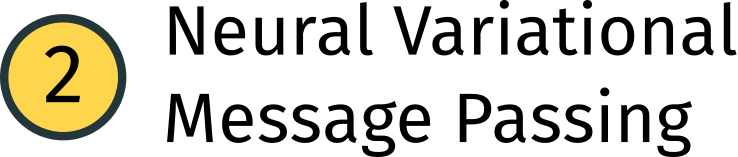
\includegraphics{img/overview-digit-2}\end{array}$
  
  \begin{itemize}
    \pause
    \item Generalizes VAE and SVAE
    \pause
    \item Extends it to new models (non-linear dynamical system, Bayesian logistic regression)
    
    \pause
    
    \item Optimizes a lower bound on the ELBO
    \pause
    \item Enables very simple software package
    \begin{center}
        \begin{figure}[H]
            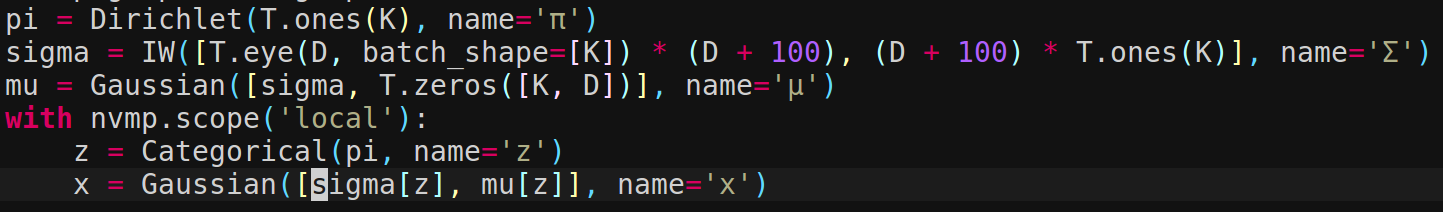
\includegraphics[width=0.8\textwidth]{img/nvmp-code}
        \end{figure}
    \end{center}
  \end{itemize}
\end{frame}

\begin{frame}{Example: Bayesian logistic regression}
  \centering
  \begin{columns}
    \begin{column}{0.3\textwidth}
      \includegraphics{tikz/blr}
    \end{column}
    \begin{column}{0.3\textwidth}
      \begin{align*}
        w &\sim \N(0, I) \\
        y_i | w, x_i &\sim \mathrm{Bernoulli}(\sigma(w^Tx_i))
      \end{align*}
    \end{column}
  \end{columns}
  \pause
  
  \alert{Problematic message:} $m^{y_i \rightarrow w}$
  \pause
  
  \textbf{Replace with:} $r_\phi(y_i, x_i)$
  
  \pause
  NVMP achieves parity with gradient descent!
\end{frame}

\begin{frame}{Overview}
  \centering
  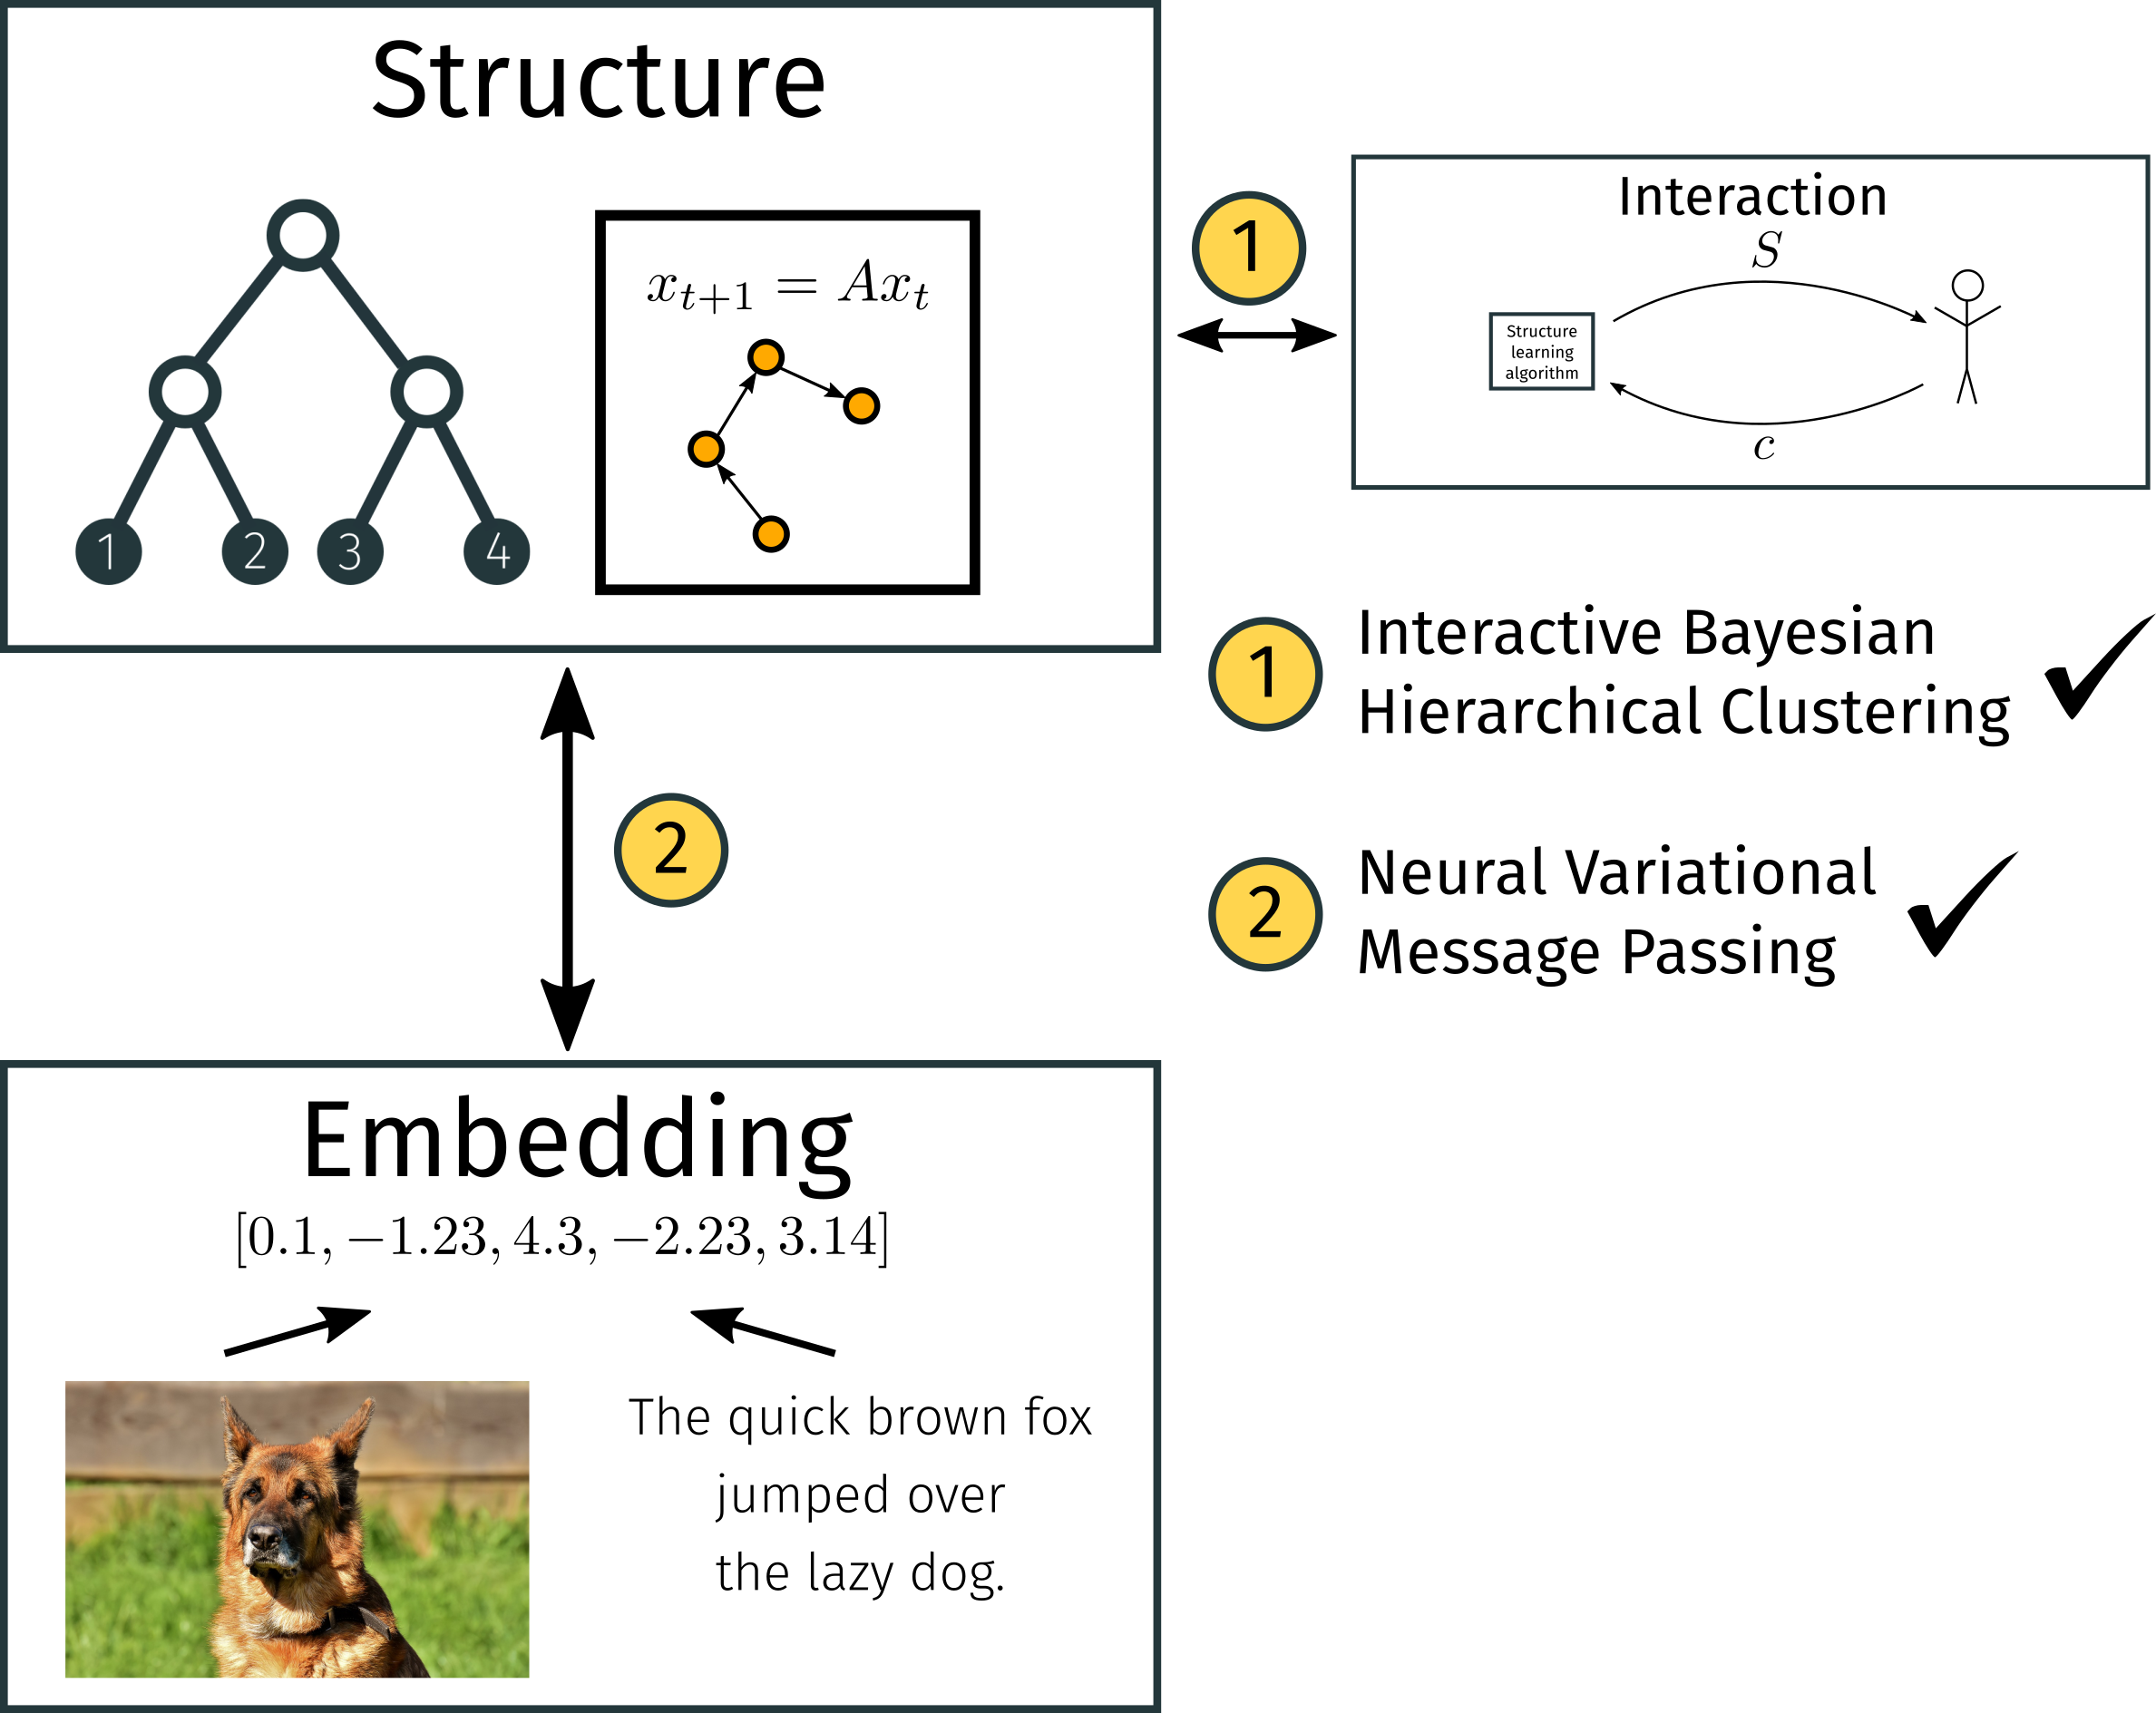
\includegraphics[width=0.8\textwidth]{img/overview-2}
\end{frame}

\section{Applications}

\begin{frame}{Model-based reinforcement learning}
    Joint work with Marvin Zhang and Sergey Levine of UC Berkeley
    \pause
    
	Consider an agent in a system,
	and a set of its possible actions.
	\begin{center}
		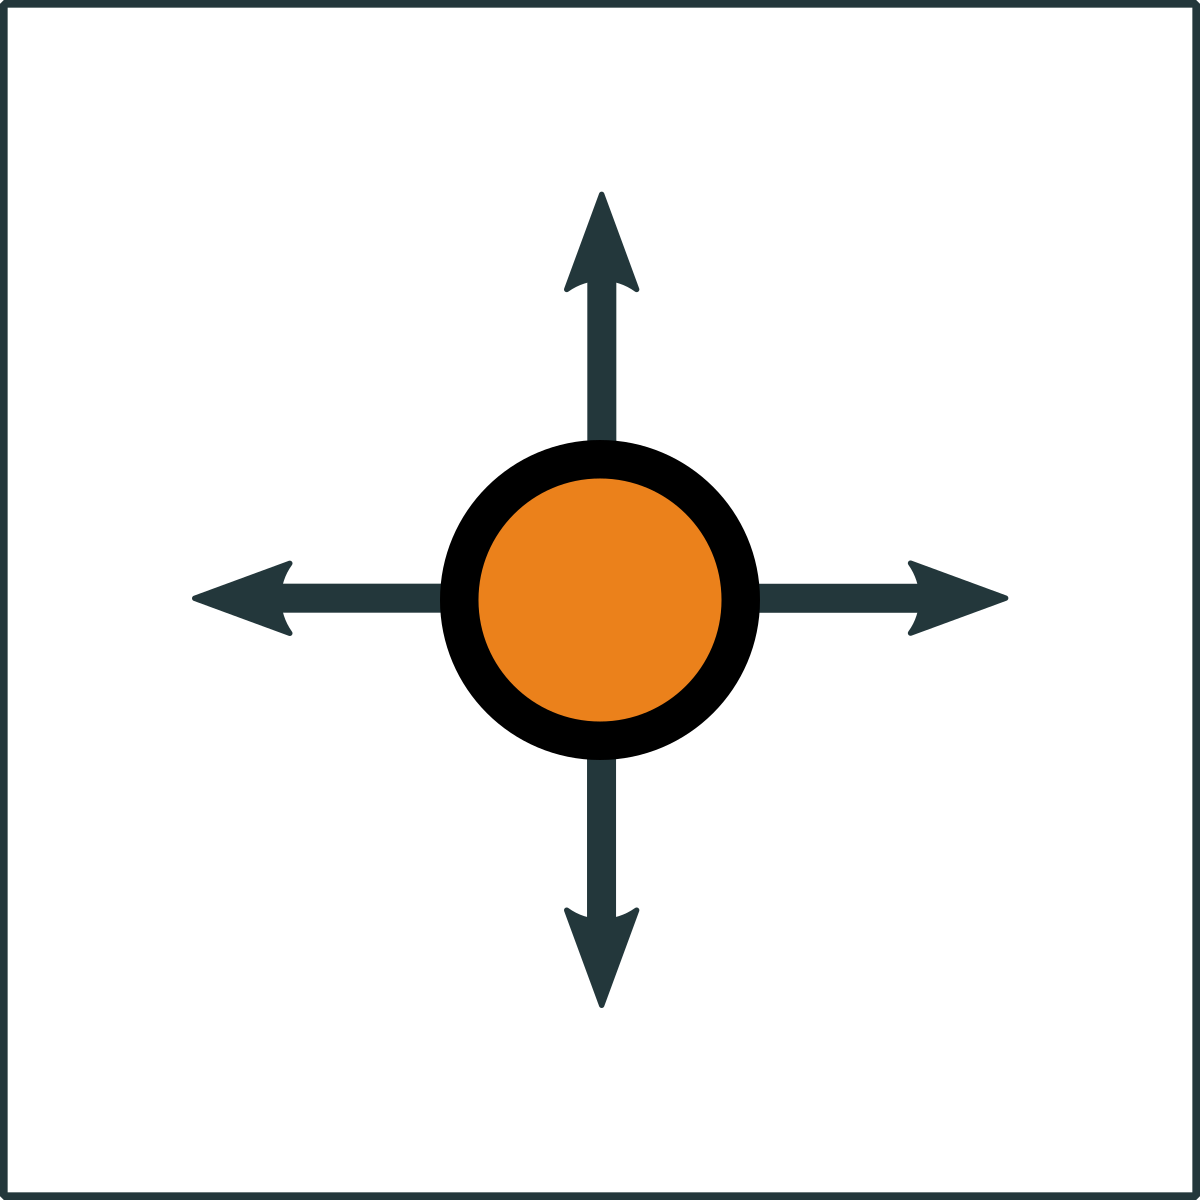
\includegraphics[width=0.5\textwidth]{img/agent-env-1.png}
	\end{center}
	\pause
	Model learning is the problem of estimating the dynamics of the system
	when we don't know it beforehand.
\end{frame}

\begin{frame}{Model learning}
	Formally, consider an agent in a system with state space $\mathcal{S}$
	with action space $\mathcal{A}$ with underlying dynamics 
	function $p(s_{t + 1} | s_t, a_t)$.

	We are interested in learning an approximate dynamics function
	\begin{align*}\hat{p}(s_{t + 1} | s_t, a_t)\end{align*}
		from a dataset of trajectories \begin{align*}\bm{\tau} = \{(s^{(i)}_0, a^{(i)}_0, s^{(i)}_1, a^{(i)}_1, \ldots, s^{(i)}_T)\}_{i = 1}^N\end{align*}
\end{frame}

\iffalse
\begin{frame}{Bayesian linear dynamical system}
  \begin{columns}
    \begin{column}{0.3\textwidth}
        \includegraphics{tikz/blds}
    \end{column}
    \begin{column}{0.3\textwidth}
      \begin{align*}
        A, \Sigma &\sim \MNIW(\Psi, \nu, M_0, V) \\
        s_{t + 1} | s_t, a_t, A, \Sigma &\sim \N(A\begin{bmatrix}s_t\\a_t\end{bmatrix}, \Sigma)
      \end{align*}
    \end{column}
  \end{columns}
	We are interested in the posterior distribution 
	$
	p(A, \Sigma | {s_0, a_0, \ldots, s_T})
	$
	which can be computed analytically.
\end{frame}
\fi

\begin{frame}{Latent linear dynamical system}
  \begin{columns}
    \begin{column}{0.3\textwidth}
        \includegraphics{tikz/lblds}
    \end{column}
    \begin{column}{0.6\textwidth}
      \begin{align*}
        A, \Sigma &\sim \MNIW(\Psi, \nu, M_0, V) \\
        x_{t + 1} | x_t, a_t, A, \Sigma &\sim \N(A\begin{bmatrix}x_t\\a_t\end{bmatrix}, \Sigma)
        s_t | x_t &\sim \N(\mu_\gamma(x_t), \Sigma_\gamma(x_t))
      \end{align*}
    \end{column}
  \end{columns}
	The posterior distribution 
	$
	q(A, \Sigma, x_0, \ldots, x_T | {s_0, a_0, \ldots, s_T})
	$
	is no longer tractable, but can be approximated via NVMP.
\end{frame}

\begin{frame}{Reinforcement learning}
    
    \begin{center}
        Learning to Model: Deep Structured Representations for Dynamics Inference in Reinforcement Learning - Zhang, Vikram, \& Levine (submitting to NIPS 2018)
        $\begin{array}{l}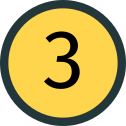
\includegraphics{img/overview-digit-3}\end{array}$
    \end{center}
    
    \pause
    High level approach:
    \begin{itemize}
    \pause
        \item Learns a mapping from non-linear dynamical system to an LDS
    \pause
        \item Model-predictive control in the latent space to minimize a cost function
    \end{itemize}
    
    \pause
    Why is this approach good?
    \begin{itemize}
        \pause
        \item Sample efficiency
        \pause
        \item Works on image-based domains and
        complex robotics tasks
    \end{itemize}
    
\end{frame}

\begin{frame}{Overview}
  \centering
  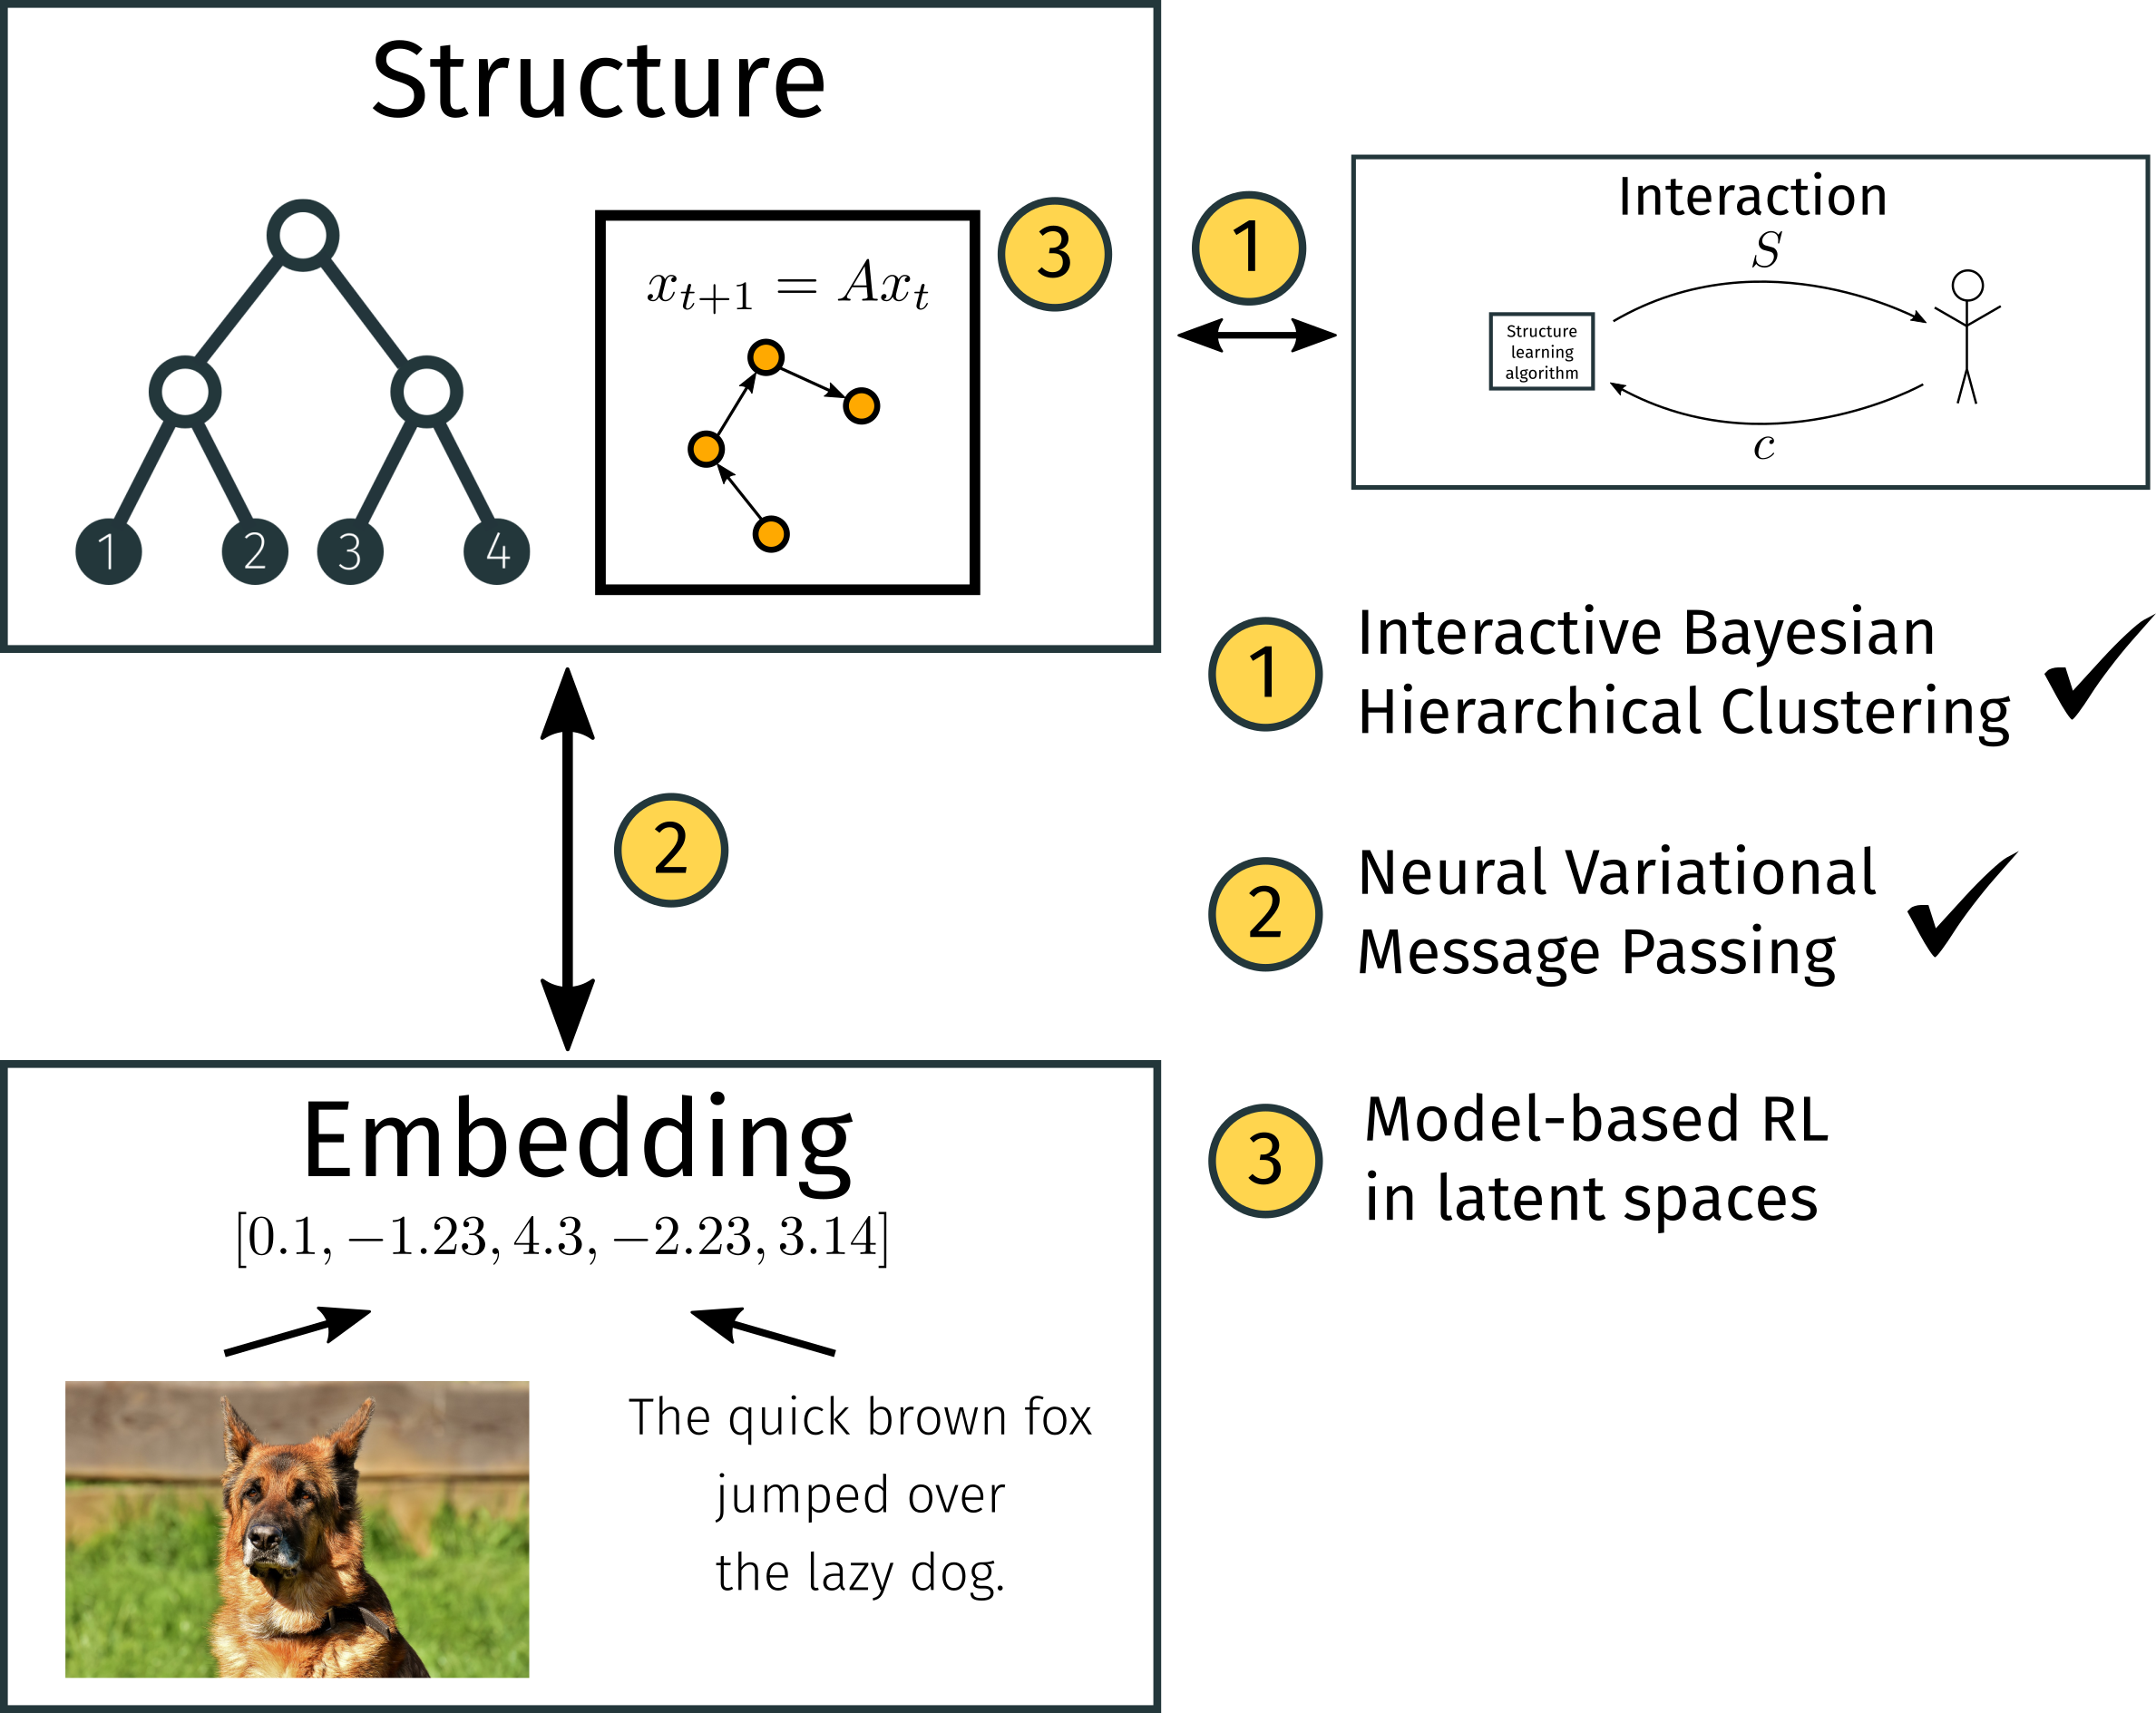
\includegraphics[width=0.8\textwidth]{img/overview-3}
\end{frame}

\begin{frame}{Hierarchical clustering in latent spaces}

    \begin{center}
        \includegraphics{tikz/ltmc}
    \end{center}
    \pause
    
    Existing work:
    \begin{itemize}
        \item Nested Chinese restaurant process - \cite{Goyal2017NonparametricLearning}
        \item Dirichlet diffusion tree - ?
        \item Kingman Coalescent - ?
        \item Time marginalized coalescent - ?
    \end{itemize}
    \pause
    
    Why? Inference in these models is harder!  $\begin{array}{l}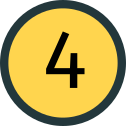
\includegraphics{img/overview-digit-4}\end{array}$
    
\end{frame}

\begin{frame}{Challenges}
    
    Most challenges in using these models come from scalability:
    
    \begin{itemize}
        \item Representing a full binary tree over a million data points isn't practical
        \item Searching the space of trees if your dataset is large is impractical
        \item How do you train a tree with minibatches? Variational inference?
        \item How do you incorporate interaction?
    \end{itemize}
    
    My solutions:
    \begin{itemize}
        \item $q(\tau)$ - pruned tree
        \item Variational particle approximation - \cite{Saeedi2014VariationalApproximations}
        \item Neural variational message passing
        \item Interaction fits in naturally with a particle approximation
    \end{itemize}
\end{frame}

\begin{frame}{Overview}
  \centering
  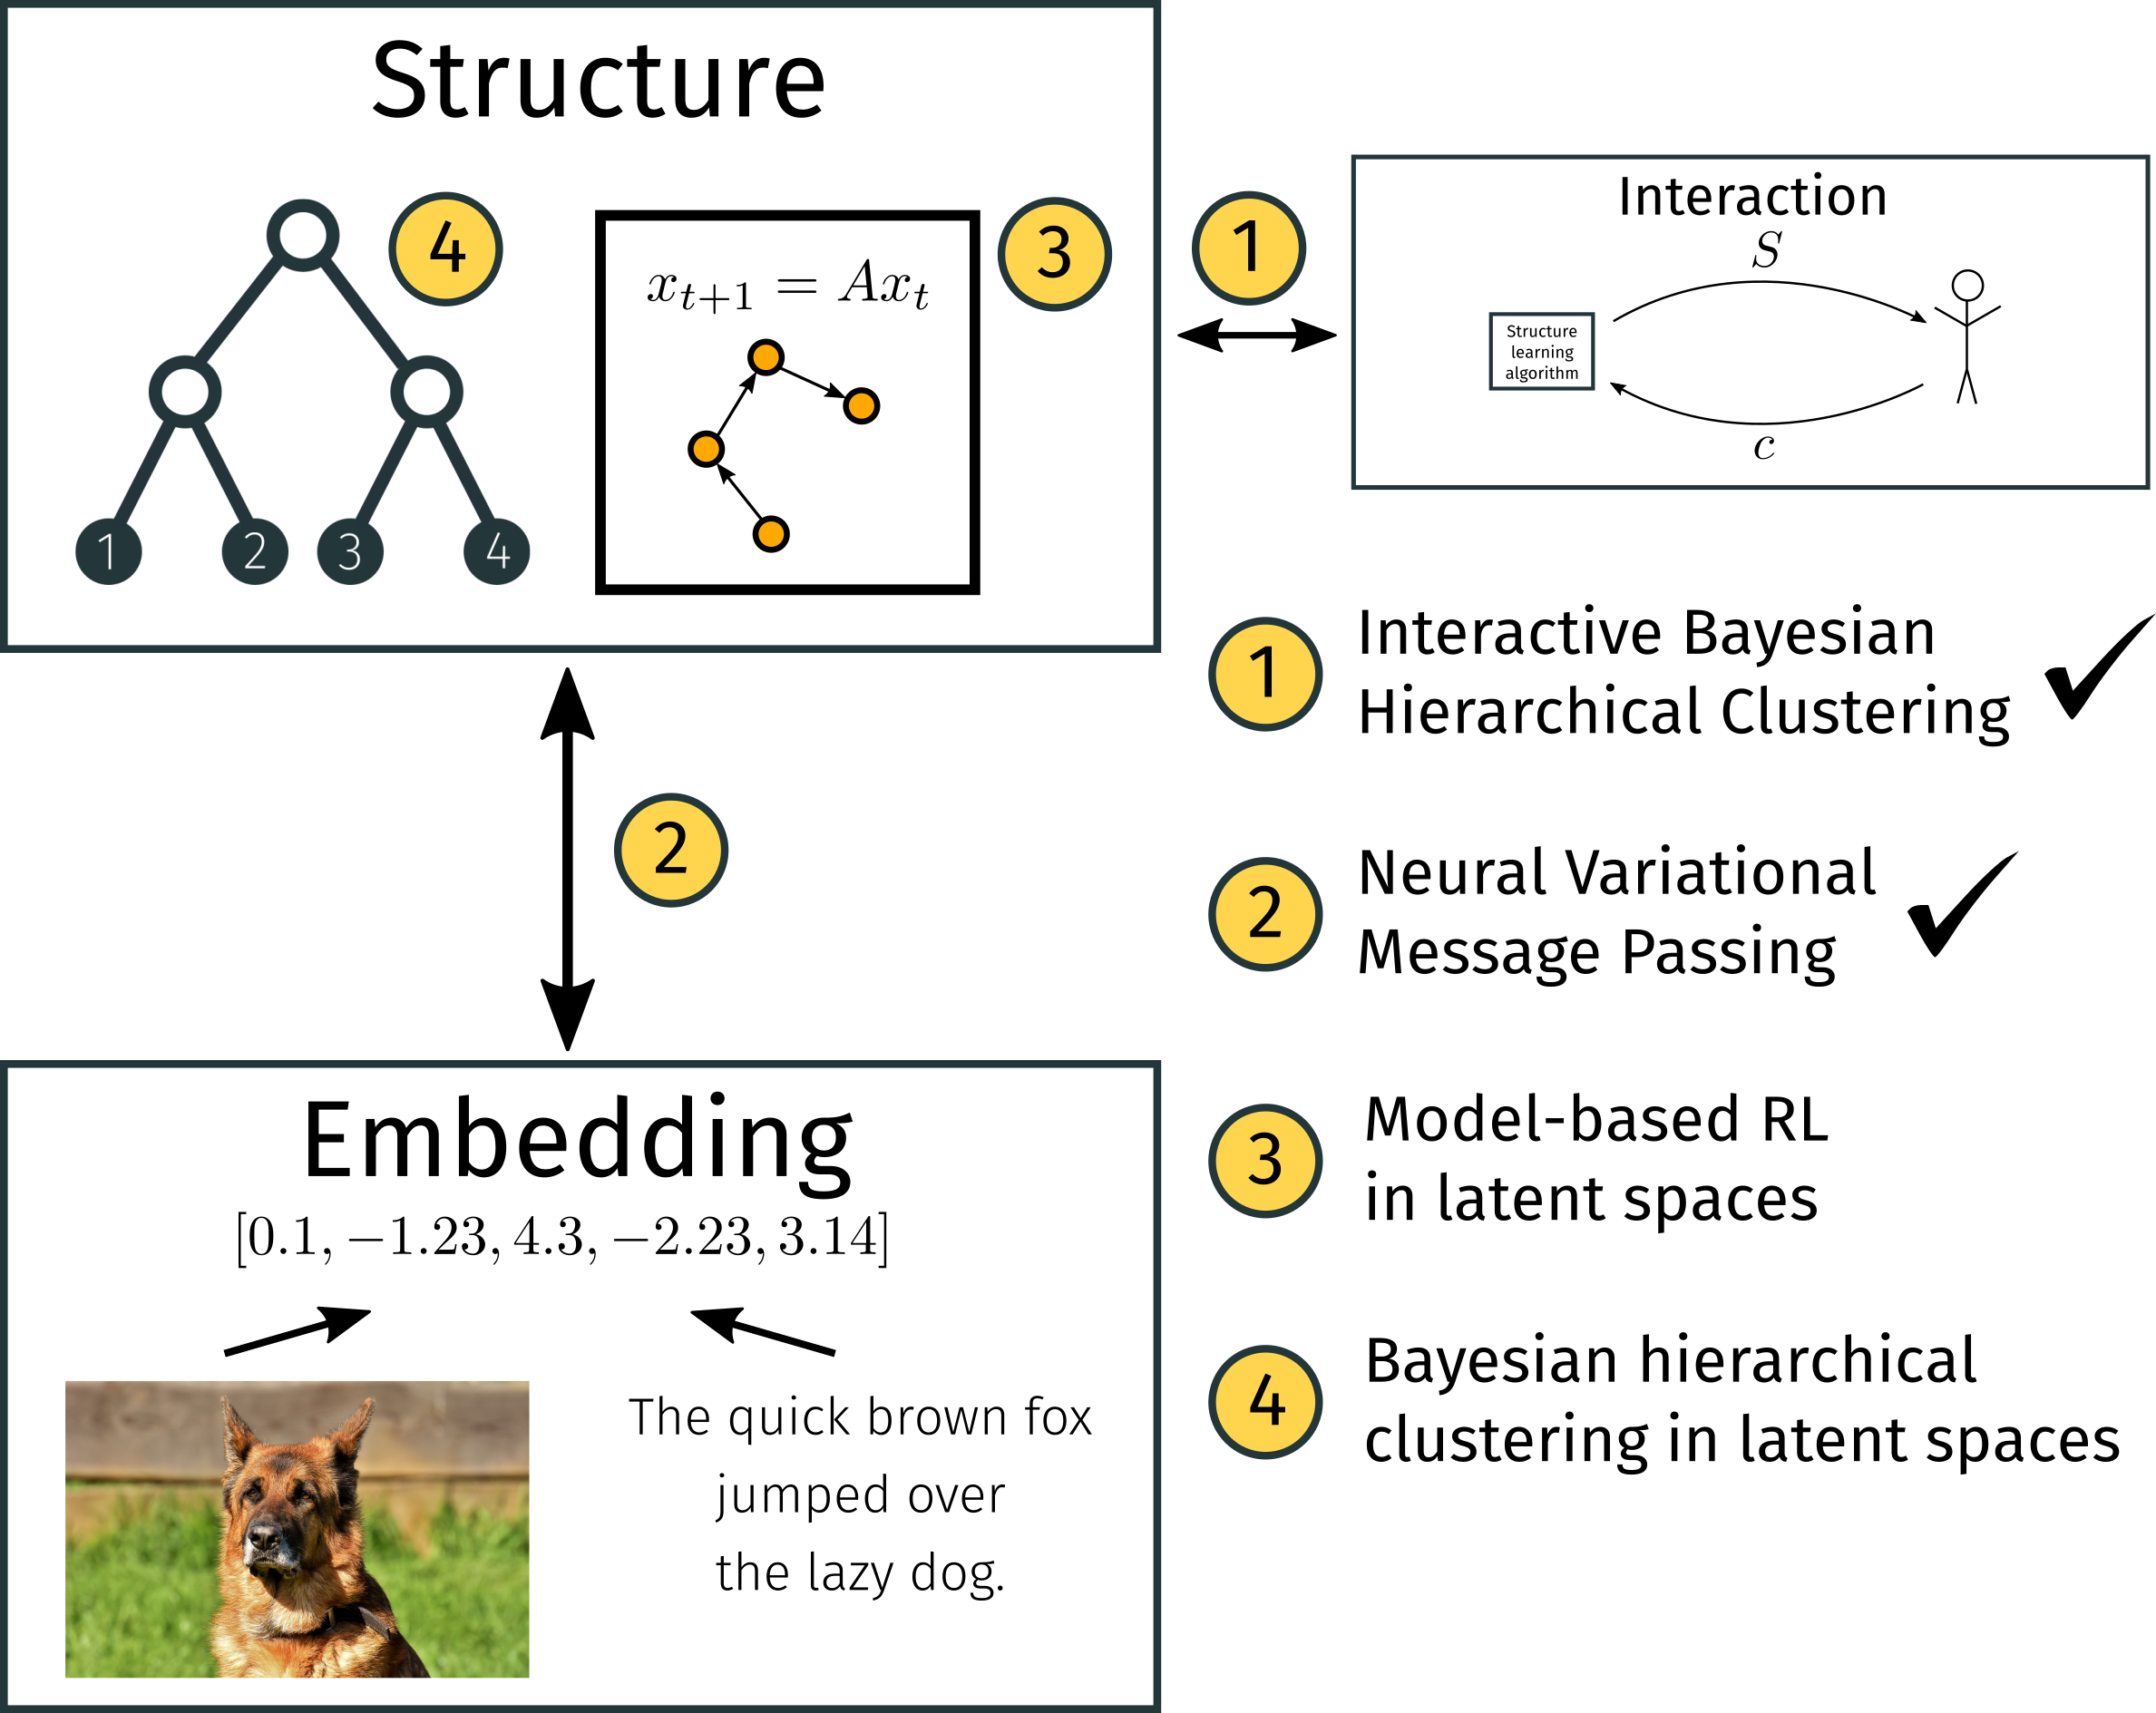
\includegraphics[width=0.8\textwidth]{img/overview-4}
\end{frame}

\begin{frame}{Future work}
    Interactive learning
    \begin{itemize}
    \pause
        \item Noisy constraints
    \pause
        \item Interactive reinforcement learning
    \pause
        \item Can interaction improve reinforcement learning?
    \end{itemize}
    
    Structure embeddings
    \begin{itemize}
    \pause
        \item Language modeling - latent Markov model
    \pause
        \item More complex dynamical systems - switching states
    \pause
        \item Automating amortized inference
    \end{itemize}
    \pause
\end{frame}

\begin{frame}[standout]
    Thank you! Any questions?
\end{frame}


\begin{frame}[allowframebreaks]{References}
    \bibliographystyle{unsrtnat}
    \bibliography{mendeley} 
\end{frame}
%\begin{frame}{Messages in SVAE}
  %The message from a \textbf{non-conjugate, non-exponential family} observation $X$ to a parent $Y$ is
  %\begin{align*}
    %m_{X \rightarrow Y} = r_\xi(t_X(X))
  %\end{align*}
  %where $r_\xi$ is a neural network whose output
  %is the same shape of a message from a conjugate-exponential child.

  %\pause
  %\metroset{block=fill}
  %\begin{block}{Inference in a SVAE}
    %\begin{enumerate}
      %\item For a data $\tau = \{s_0, a_0, s_1, a_1, \ldots, s_T\}$,
        %perform VMP using SVAE messages
      %\item Compute the ELBO $\L[q(\{x_i\}_{i = 1}^T, \mu_{\isdmodel}, \Sigma_{\isdmodel}, \dynmat, \dyncovar)]$
      %\item Update neural networks with $\nabla_{\gamma, \xi} \L[q(\{x_i\}_{i = 1}^T, \mu_{\isdmodel}, \Sigma_{\isdmodel}, \dynmat, \dyncovar)]$
      %\item Update global parameters ($\mu_{\isdmodel}, \Sigma_{\isdmodel}, \dynmat, \dyncovar$) with natural gradients
    %\end{enumerate}
  %\end{block}
%\end{frame}
\appendix
\begin{frame}{Intelligent subset queries}

  Recall the interaction model.

  \begin{center}
    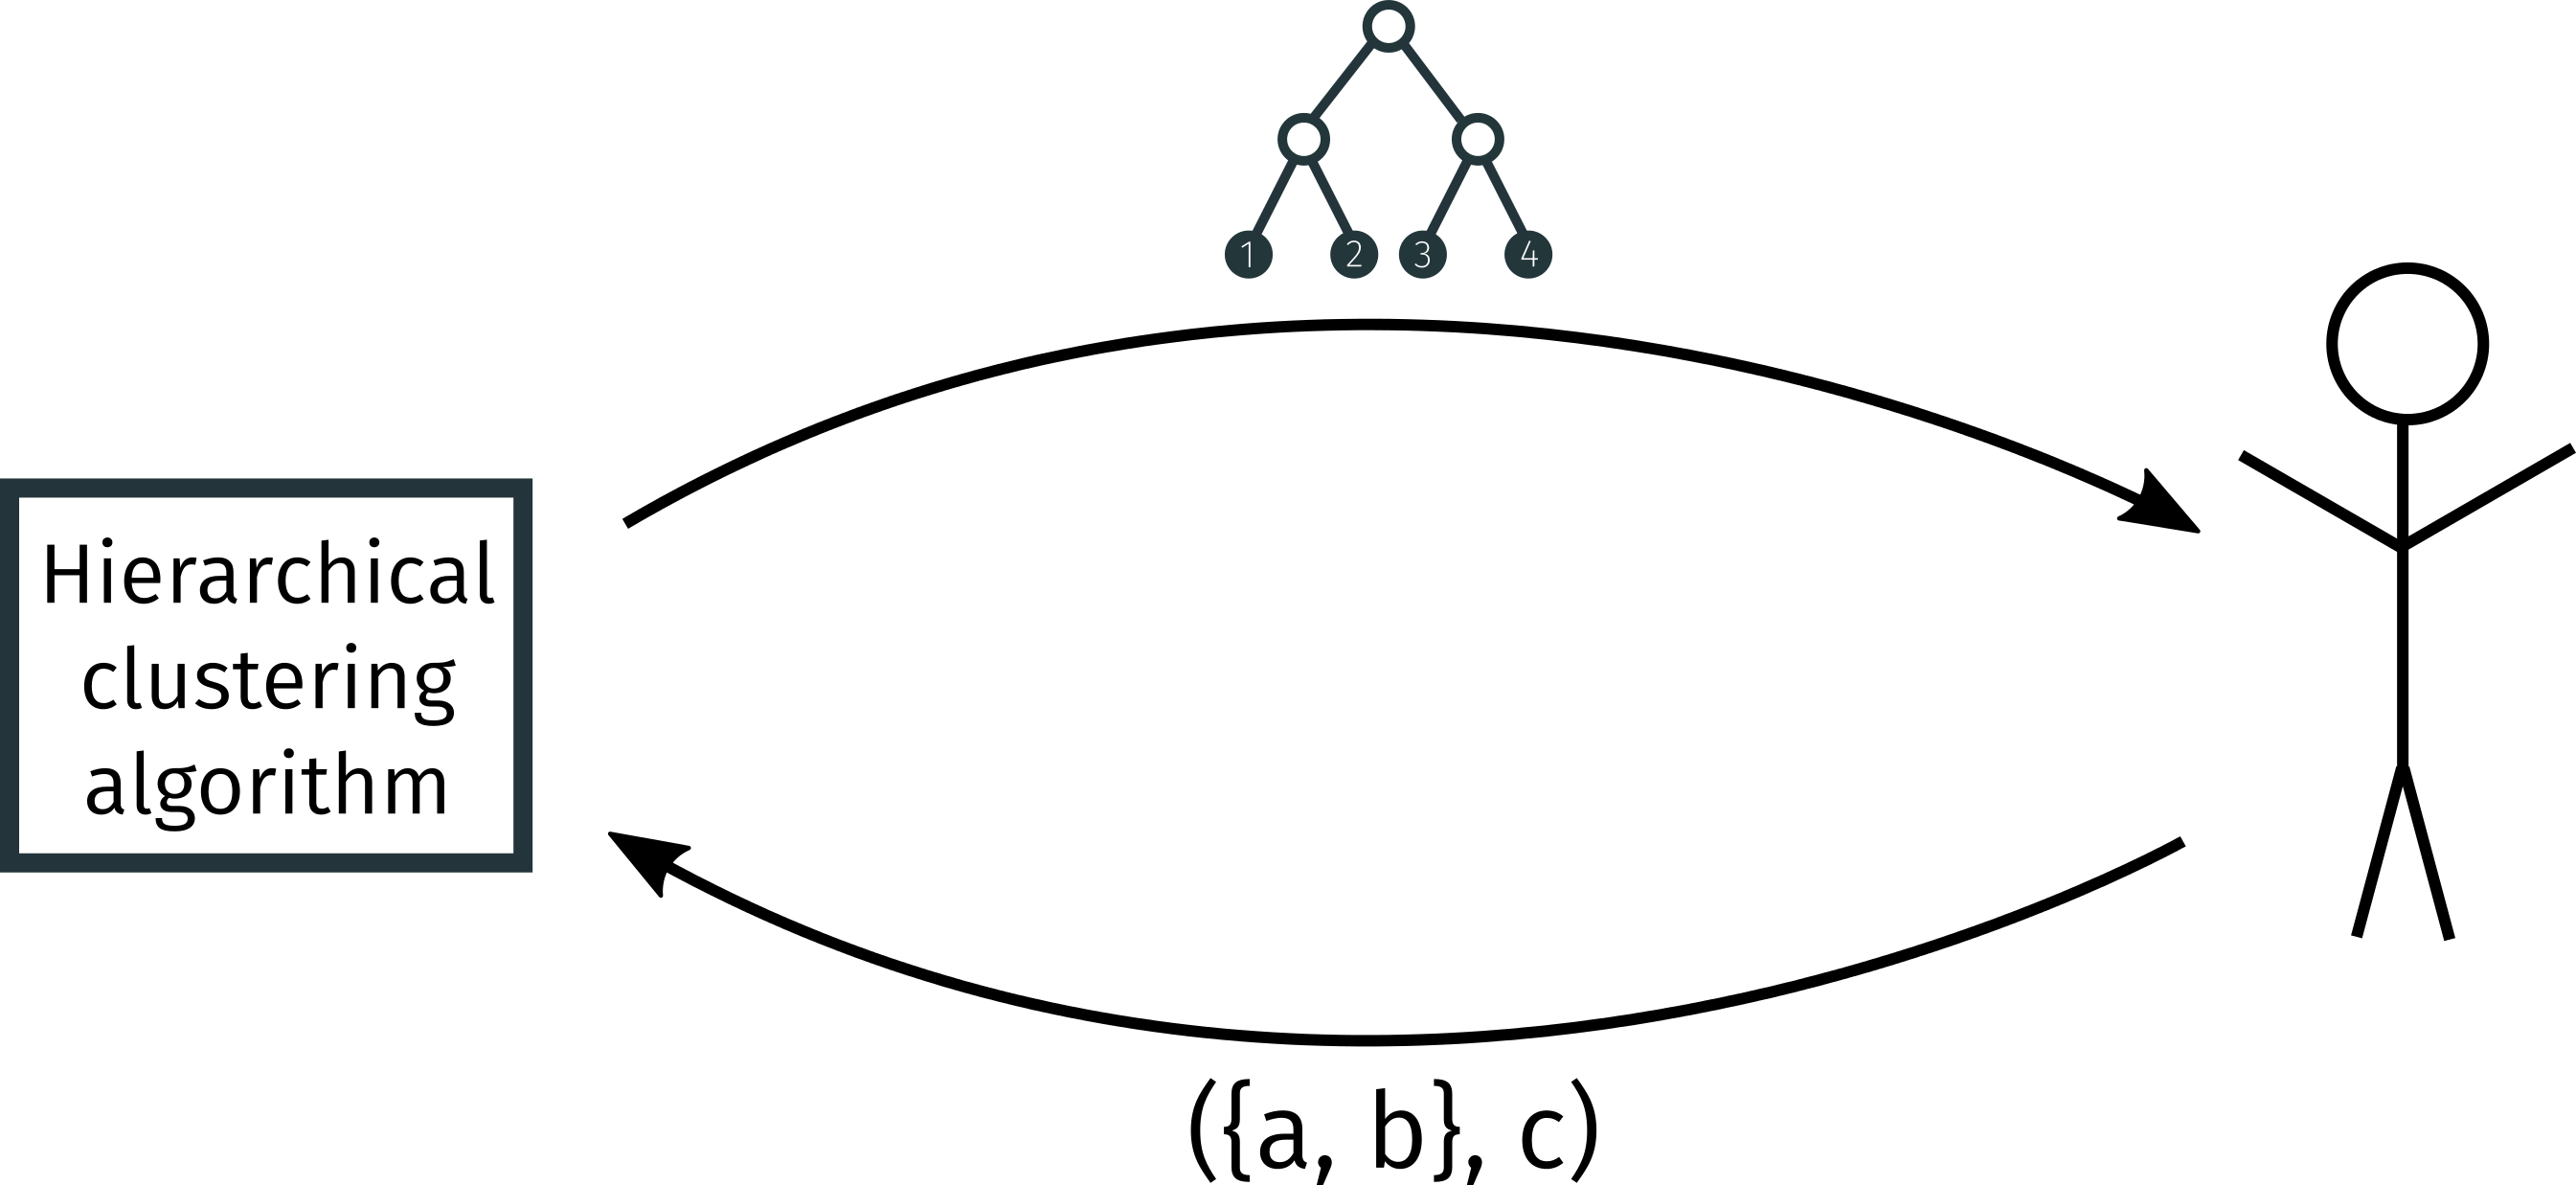
\includegraphics[width=\textwidth]{img/interaction-3}
  \end{center}

  \pause

  %We pick a subset of data $S$ and show a user the candidate tree
  %restricted to $S$, $T|_S$.

  %\pause

  \textbf{Idea:}  pick subsets that have high variance
  under the posterior distribution

\end{frame}

\begin{frame}{Measuring subtree variance}

    First, sample $N$ trees from posterior distribution.

  \pause

 \metroset{block=fill}
  \begin{block}{Definition: tree distance variance (TDV)}
    Given a subset of data $S$ and tree samples $\mathcal{T} = T_1, \ldots, T_N$,
    \begin{align}
      \mathrm{TDV}(S, \mathcal{T}) = \max_{i, j \in S}  \mathrm{Var}_{T \in \mathcal{T}}\left[\texttt{tree-dist}_{T|S}(i, j)\right]
    \end{align}
  where $\texttt{tree-dist}_T$ is the number of edges needed to get from leaf $i$ to leaf $j$
  in tree $T$.
  \end{block}

  \pause

Instantiate $L$ subsets randomly and pick the one with the highest variance.

\end{frame}

\begin{frame}{KL-divergence}
  Kullback-Leibler (KL) divergence
  is a measure of how far one probability distribution
  is from another.

  \pause
  For distributions $q(x)$ and $p(x)$,
  \begin{align*}
    \textrm{KL}(q(x)\|p(x)) = \int q(x)\log \frac{q(x)}{p(x)}dx = \E_{q(x)}\left[\log\frac{q(x)}{p(x)}\right]
  \end{align*}

  \pause
  \textbf{Properties:}
  \begin{itemize}
    \item $\textrm{KL}(q(x)\|p(x)) = 0$ if $q(x) = p(x)$.
    \item Asymmetric
  \end{itemize}
\end{frame}

\begin{frame}{Exponential family}
  A probability distribution is in the \emph{exponential family}
  if it can be parametrized in the following way.

  \pause

  \begin{align*}
    \log p(y | x) = \left\langle\eta(x), t_y(y)\right\rangle - \log Z(\eta(x))
  \end{align*}
  where
  \begin{itemize}
      \pause
    \item $\eta(x)$ - natural parameter function
      \pause
    \item $t_y(y)$ - sufficient statistic function
      \pause
    \item $\log Z(\eta(x))$ - log-partition function
  \end{itemize}
  \pause
  \textbf{Examples:} Gaussian, Categorical, Dirichlet, inverse-Wishart
\end{frame}

\begin{frame}{Conjugacy}
   \begin{center}
        \includegraphics{tikz/conjugate-pair}
   \end{center}
   A pair of random variables are conjugate if
   you can rearrange $p(y | x)$ from

  \pause

  \begin{align*}
    \log p(x) &= \left\langle\eta_x, t_x(x)\right\rangle - \log Z(\eta_x) \\
    \log p(y | x) &= \left\langle\eta_y(x), t_y(y)\right\rangle - \log Z(\eta_y(x))
  \end{align*}
  to
  \pause
  \begin{align*}
    \log p(y | x) \propto \left\langle t_x(x), \eta^*_y(y)\right\rangle
  \end{align*}
\end{frame}

\begin{frame}{Posterior distribution}
   \begin{center}
        \includegraphics{tikz/conjugate-pair}
   \end{center}
  \begin{align*}
    \log p(y | x) \propto \left\langle t_x(x), \eta^*_y(y)\right\rangle
  \end{align*}
  \pause
  The corresponding posterior distribution is:
  \begin{align*}
    \log p(x | y) = \left\langle t_x(x), \eta^*_y(y) + \eta_x\right\rangle + \log Z(\eta^*_y(y) + \eta_x)
  \end{align*}
  \pause
  \centering
  \fbox{
      \scalebox{2}{$\eta^*_y(y) + \eta_x$}
  }
\end{frame}

\begin{frame}{Messages}
  Remember that $\eta_j$ is the natural parameter of the distribution $q(\mathbf{H}_j)$.
  \pause
  The message from a parent $Y$ to a child $X$ is
  \begin{align*}
    m_{Y \rightarrow X} = f(\eta_Y)
  \end{align*}
  \pause
  The message from a child $X$ to a parent $Y$ is
  \begin{align*}
    m_{X \rightarrow Y} = g(\eta_X, \{m_{i \rightarrow X}\}_{i \in \textrm{cp}_Y})
  \end{align*}

  \pause
  In conjugate-exponential PGMs, messages can be computed in closed-form.
\end{frame}

\begin{frame}{Summary of VMP}
  \textbf{Setup:} Conjugate-exponential graphical model

  \pause
  \textbf{Problem:} Compute posterior $p(\mathbf{H} | \mathbf{V})$, approximated with $q(\mathbf{H}) = \prod_j q(\mathbf{H}_j)$

  \pause
  \textbf{Solution:} Until converged, for each hidden node $\mathbf{H}_j$:
  \begin{enumerate}
    \pause
  \item Collect messages from children and parents
    \pause
  \item Compute updated distribution parameters from messages
\end{enumerate}

\pause
\textbf{Benefits:} efficient, simple, can incorporate mini-batches (stochastic variational inference)

\pause
\textbf{Drawbacks:} can be underexpressive (conjugate-exponential requirement)
\end{frame}


\end{document}